% Requires in the preamble:
% \usepackage{amsmath,amssymb}
% \usepackage{tikz,pgfplots}
% \pgfplotsset{compat=1.18}

\chapter{Complex Numbers, Fourier Series, and the Road Ahead}
\label{chap:complex-fourier-road-ahead}

The last chapter ended with a strange-looking promise:

\[
e^{i\theta}=\cos\theta+i\sin\theta.
\]

The formula says that an exponential can trace a circle.  At first that sounds impossible.
Exponential growth moves away from \(0\).  Sine and cosine move back and forth.  A
circle turns.  Why should one formula connect all three?

Taylor series gave the clue.  The series for \(e^x\), \(\cos x\), and \(\sin x\) have the
same factorials hiding inside them.  The missing ingredient is a number whose square is

\[
-1.
\]

That number is called \(i\).  It opens a new plane of numbers, and in that plane the
exponential becomes the natural language of rotation.

\section{Complex numbers and Euler's formula}
\label{sec:complex-numbers-euler-formula}

The real number line is one-dimensional.  It can measure position to the left and right,
size, error, and signed change.  But it cannot solve

\[
x^2+1=0.
\]

No real number has square \(-1\).

Instead of giving up, mathematics enlarges the number system.

\subsection{The complex plane}
\label{subsec:complex-plane}

Define a new number \(i\) by the rule

\[
\boxed{i^2=-1.}
\]

A \emph{complex number} is a number of the form

\[
\boxed{z=a+bi,}
\]

where \(a\) and \(b\) are real numbers.

The number \(a\) is called the \emph{real part} of \(z\), and \(b\) is called the
\emph{imaginary part} of \(z\):

\[
\operatorname{Re}(z)=a,
\qquad
\operatorname{Im}(z)=b.
\]

For example,

\[
z=3+4i
\]

has

\[
\operatorname{Re}(z)=3,
\qquad
\operatorname{Im}(z)=4.
\]

A complex number can be drawn as a point in a plane.  The horizontal axis records the
real part.  The vertical axis records the imaginary part.

\begin{figure}[h]
\centering
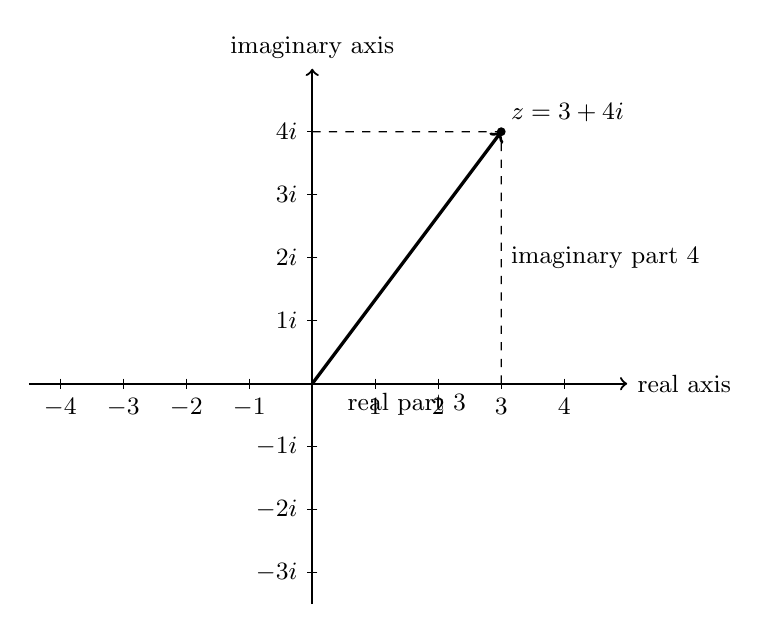
\begin{tikzpicture}[scale=0.8, every node/.style={font=\small}]
  \draw[->, thick] (-4.5,0) -- (5,0) node[right] {real axis};
  \draw[->, thick] (0,-3.5) -- (0,5) node[above] {imaginary axis};

  \foreach \x in {-4,-3,-2,-1,1,2,3,4} {
    \draw (\x,0.08) -- (\x,-0.08);
    \node[below] at (\x,-0.08) {\(\x\)};
  }

  \foreach \y in {-3,-2,-1,1,2,3,4} {
    \draw (0.08,\y) -- (-0.08,\y);
    \node[left] at (-0.08,\y) {\(\y i\)};
  }

  \coordinate (Z) at (3,4);
  \draw[very thick,->] (0,0) -- (Z);
  \draw[dashed] (3,0) -- (Z);
  \draw[dashed] (0,4) -- (Z);
  \fill (Z) circle (2pt);

  \node[above right] at (Z) {\(z=3+4i\)};
  \node[below] at (1.5,0) {real part \(3\)};
  \node[right] at (3,2) {imaginary part \(4\)};
\end{tikzpicture}
\caption{The complex number \(3+4i\) is drawn as the point \((3,4)\) in the complex plane.}
\label{fig:complex-plane-3-plus-4i}
\end{figure}

Addition works just like vector addition:

\[
(a+bi)+(c+di)=(a+c)+(b+d)i.
\]

Subtraction is the same:

\[
(a+bi)-(c+di)=(a-c)+(b-d)i.
\]

Multiplication uses the single rule \(i^2=-1\):

\[
(a+bi)(c+di)
=
ac+adi+bci+bdi^2.
\]

Since \(i^2=-1\),

\[
\boxed{
(a+bi)(c+di)=(ac-bd)+(ad+bc)i.
}
\]

\paragraph{Example.}
Multiply

\[
(2+3i)(4-i).
\]

We compute

\[
(2+3i)(4-i)
=
8-2i+12i-3i^2.
\]

Since \(i^2=-1\),

\[
-3i^2=3.
\]

Thus

\[
(2+3i)(4-i)=11+10i.
\]

Complex arithmetic is ordinary algebra, together with the rule \(i^2=-1\).

\begin{quote}
\textbf{Complex conjugate and modulus.}
If

\[
z=a+bi,
\]

then its \emph{complex conjugate} is

\[
\boxed{\overline{z}=a-bi.}
\]

Its \emph{modulus} is its distance from \(0\) in the complex plane:

\[
\boxed{|z|=\sqrt{a^2+b^2}.}
\]
\end{quote}

The conjugate reflects a complex number across the real axis.

The modulus is the length of the vector from \(0\) to \(z\).  For \(z=3+4i\),

\[
|z|=\sqrt{3^2+4^2}=5.
\]

The conjugate and modulus are connected by a useful identity:

\[
z\overline{z}=(a+bi)(a-bi).
\]

Multiplying,

\[
z\overline{z}
=
a^2-ab i+ab i-b^2 i^2
=
a^2+b^2.
\]

Therefore

\[
\boxed{
z\overline{z}=|z|^2.
}
\]

This identity lets us divide complex numbers.

\paragraph{Example.}
Simplify

\[
\frac{1}{3+4i}.
\]

Multiply numerator and denominator by the conjugate:

\[
\frac{1}{3+4i}
=
\frac{1}{3+4i}\cdot\frac{3-4i}{3-4i}.
\]

Then

\[
(3+4i)(3-4i)=3^2+4^2=25.
\]

So

\[
\boxed{
\frac{1}{3+4i}=\frac{3-4i}{25}
=
\frac{3}{25}-\frac{4}{25}i.
}
\]

The complex plane now gives \(i\) a geometric meaning.  The number \(i\) is the point

\[
0+1i.
\]

It is one unit above the origin.  Multiplication by \(i\) will turn out to mean a
quarter-turn rotation.

\subsection{Polar form}
\label{subsec:complex-polar-form}

A nonzero point in the plane can be described in two ways.

We can give its horizontal and vertical coordinates:

\[
z=a+bi.
\]

Or we can give its distance from the origin and its angle from the positive real axis.

Let

\[
r=|z|=\sqrt{a^2+b^2}.
\]

If \(z\neq0\), choose an angle \(\theta\) so that

\[
a=r\cos\theta,
\qquad
b=r\sin\theta.
\]

Then

\[
z=a+bi
=
r\cos\theta+i r\sin\theta.
\]

So

\[
\boxed{
z=r(\cos\theta+i\sin\theta).
}
\]

This is called the \emph{polar form} of \(z\).

\begin{figure}[h]
\centering
\begin{tikzpicture}[scale=2.1, every node/.style={font=\small}]
  \draw[->] (-1.35,0) -- (2.1,0) node[right] {real};
  \draw[->] (0,-0.45) -- (0,1.55) node[above] {imaginary};

  \def\r{1.55}
  \def\ang{35}
  \coordinate (Z) at ({\r*cos(\ang)},{\r*sin(\ang)});

  \draw[very thick,->] (0,0) -- (Z);
  \draw[dashed] ({\r*cos(\ang)},0) -- (Z);
  \draw[dashed] (0,{\r*sin(\ang)}) -- (Z);

  \draw[thick] (0.42,0) arc (0:\ang:0.42);
  \node at ({0.58*cos(18)},{0.58*sin(18)}) {\(\theta\)};

  \node[above right] at (Z) {\(z=a+bi\)};
  \node[below] at ({\r*cos(\ang)/2},0) {\(a=r\cos\theta\)};
  \node[left] at (0,{\r*sin(\ang)/2}) {\(b=r\sin\theta\)};
  \node[above left] at ({0.72*cos(\ang)},{0.72*sin(\ang)}) {\(r=|z|\)};
\end{tikzpicture}
\caption{Polar form records a complex number by its length \(r\) and angle \(\theta\).}
\label{fig:complex-polar-form}
\end{figure}

The angle \(\theta\) is called an \emph{argument} of \(z\).

There is one warning: angles are not unique.  Turning once around the circle does not
change the point.  Thus

\[
\theta,\quad \theta+2\pi,\quad \theta-2\pi,\quad \theta+4\pi,\ldots
\]

all describe the same direction.

So a nonzero complex number has many polar forms:

\[
r(\cos\theta+i\sin\theta)
=
r(\cos(\theta+2\pi k)+i\sin(\theta+2\pi k)),
\qquad k\in\mathbb Z.
\]

The number \(0\) has modulus \(0\), but it has no preferred angle.  Every direction
points away from the origin, and \(0\) is not away from the origin.

\paragraph{Example.}
Write

\[
1+i
\]

in polar form.

Its modulus is

\[
r=\sqrt{1^2+1^2}=\sqrt2.
\]

Its angle is

\[
\theta=\frac{\pi}{4}.
\]

Therefore

\[
\boxed{
1+i=\sqrt2\left(\cos\frac{\pi}{4}+i\sin\frac{\pi}{4}\right).
}
\]

\paragraph{Example.}
Write

\[
-2
\]

in polar form.

This point lies on the negative real axis.  Its modulus is

\[
r=2.
\]

One argument is

\[
\theta=\pi.
\]

So

\[
\boxed{
-2=2(\cos\pi+i\sin\pi).
}
\]

We could also use \(\theta=-\pi\), or \(\theta=3\pi\).  The polar form is not unique
because angle is not unique.

\subsection{Multiplication as rotation and scaling}
\label{subsec:complex-multiplication-rotation-scaling}

Complex addition is like vector addition.  Complex multiplication is more surprising.

Take two nonzero complex numbers in polar form:

\[
z=r(\cos\theta+i\sin\theta),
\]

\[
w=s(\cos\phi+i\sin\phi).
\]

Then

\[
zw
=
rs(\cos\theta+i\sin\theta)(\cos\phi+i\sin\phi).
\]

Multiply:

\[
zw
=
rs\Bigl[
\cos\theta\cos\phi
-\sin\theta\sin\phi
+i(\sin\theta\cos\phi+\cos\theta\sin\phi)
\Bigr].
\]

Using the angle addition identities,

\[
\cos(\theta+\phi)=\cos\theta\cos\phi-\sin\theta\sin\phi,
\]

and

\[
\sin(\theta+\phi)=\sin\theta\cos\phi+\cos\theta\sin\phi,
\]

we get

\[
\boxed{
zw
=
rs\bigl(\cos(\theta+\phi)+i\sin(\theta+\phi)\bigr).
}
\]

So multiplication has a geometric meaning:

\[
\boxed{
\text{moduli multiply, and arguments add.}
}
\]

In words:

\[
\boxed{
\text{Complex multiplication scales and rotates.}
}
\]

\begin{quote}
\textbf{Multiplication in polar form.}
If

\[
z=r(\cos\theta+i\sin\theta),
\qquad
w=s(\cos\phi+i\sin\phi),
\]

then

\[
\boxed{
zw=rs\bigl(\cos(\theta+\phi)+i\sin(\theta+\phi)\bigr).
}
\]
\end{quote}

\paragraph{Example: multiplying by \(i\).}
The number \(i\) has polar form

\[
i=\cos\frac{\pi}{2}+i\sin\frac{\pi}{2}.
\]

Multiplying by \(i\) preserves length and adds angle \(\pi/2\).  Therefore multiplication
by \(i\) rotates every complex number counterclockwise by \(90^\circ\).

Algebra confirms this.  If

\[
z=a+bi,
\]

then

\[
iz=i(a+bi)=ai+b i^2=-b+ai.
\]

So

\[
\boxed{
i(a+bi)=-b+ai.
}
\]

The point \((a,b)\) becomes \((-b,a)\), which is a \(90^\circ\) counterclockwise
rotation.

\begin{figure}[h]
\centering
\begin{tikzpicture}[scale=0.95, every node/.style={font=\small}]
  \draw[->, thick] (-4.2,0) -- (4.5,0) node[right] {real};
  \draw[->, thick] (0,-3.3) -- (0,4.3) node[above] {imaginary};

  \coordinate (Z) at (3,1);
  \coordinate (IZ) at (-1,3);

  \draw[very thick,->] (0,0) -- (Z);
  \draw[very thick,->] (0,0) -- (IZ);

  \draw[thick,->] (1.0,0.33) arc (18.4:108.4:1.05);

  \fill (Z) circle (2pt);
  \fill (IZ) circle (2pt);

  \node[right] at (Z) {\(z=3+i\)};
  \node[above left] at (IZ) {\(iz=-1+3i\)};
  \node at (0.9,1.2) {\(\frac{\pi}{2}\) rotation};

  \draw[dashed] (3,0) -- (Z);
  \draw[dashed] (0,1) -- (Z);
  \draw[dashed] (-1,0) -- (IZ);
  \draw[dashed] (0,3) -- (IZ);
\end{tikzpicture}
\caption{Multiplication by \(i\) rotates a complex number counterclockwise by \(90^\circ\).}
\label{fig:multiply-by-i-rotation}
\end{figure}

\paragraph{Example.}
Compute the product

\[
\left(\sqrt2\left(\cos\frac{\pi}{4}+i\sin\frac{\pi}{4}\right)\right)
\left(3\left(\cos\frac{\pi}{6}+i\sin\frac{\pi}{6}\right)\right).
\]

The moduli multiply:

\[
\sqrt2\cdot 3=3\sqrt2.
\]

The angles add:

\[
\frac{\pi}{4}+\frac{\pi}{6}
=
\frac{3\pi}{12}+\frac{2\pi}{12}
=
\frac{5\pi}{12}.
\]

Therefore

\[
\boxed{
zw=3\sqrt2\left(\cos\frac{5\pi}{12}+i\sin\frac{5\pi}{12}\right).
}
\]

Polar form turns multiplication into geometry.  This is the reason complex numbers are
so useful for oscillation: oscillation is repeated rotation.

\subsection{Euler's formula from Taylor series}
\label{subsec:euler-formula-from-taylor-series}

The last chapter gave the Taylor series

\[
e^x
=
1+x+\frac{x^2}{2!}+\frac{x^3}{3!}
+\frac{x^4}{4!}+\cdots,
\]

\[
\cos x
=
1-\frac{x^2}{2!}+\frac{x^4}{4!}
-\frac{x^6}{6!}+\cdots,
\]

and

\[
\sin x
=
x-\frac{x^3}{3!}+\frac{x^5}{5!}
-\frac{x^7}{7!}+\cdots.
\]

We now define the complex exponential by the same power series:

\[
\boxed{
e^z=\sum_{n=0}^{\infty}\frac{z^n}{n!}
}
\]

for a complex number \(z\).

The same factorial growth that made the real exponential series converge also makes
this complex series converge.  The modulus of \(z^n/n!\) is

\[
\frac{|z|^n}{n!},
\]

and factorials eventually dominate fixed powers.

Now put

\[
z=i\theta.
\]

Then

\[
e^{i\theta}
=
1+i\theta+\frac{(i\theta)^2}{2!}
+\frac{(i\theta)^3}{3!}
+\frac{(i\theta)^4}{4!}
+\frac{(i\theta)^5}{5!}
+\cdots.
\]

The powers of \(i\) cycle:

\[
i^0=1,
\qquad
i^1=i,
\qquad
i^2=-1,
\qquad
i^3=-i,
\qquad
i^4=1.
\]

So the even powers contribute real terms:

\[
1-\frac{\theta^2}{2!}+\frac{\theta^4}{4!}
-\frac{\theta^6}{6!}+\cdots,
\]

and the odd powers contribute imaginary terms:

\[
i\left(
\theta-\frac{\theta^3}{3!}+\frac{\theta^5}{5!}
-\frac{\theta^7}{7!}+\cdots
\right).
\]

Thus

\[
e^{i\theta}
=
\left(
1-\frac{\theta^2}{2!}+\frac{\theta^4}{4!}
-\frac{\theta^6}{6!}+\cdots
\right)
+
i\left(
\theta-\frac{\theta^3}{3!}+\frac{\theta^5}{5!}
-\frac{\theta^7}{7!}+\cdots
\right).
\]

The first series is \(\cos\theta\).  The second series is \(\sin\theta\).  Therefore

\[
\boxed{
e^{i\theta}=\cos\theta+i\sin\theta.
}
\]

This is \emph{Euler's formula}.

\begin{quote}
\textbf{Euler's formula.}
For every real \(\theta\),

\[
\boxed{
e^{i\theta}=\cos\theta+i\sin\theta.
}
\]
\end{quote}

The formula gives a compact polar form:

\[
\boxed{
r(\cos\theta+i\sin\theta)=re^{i\theta}.
}
\]

So every nonzero complex number can be written as

\[
\boxed{
z=re^{i\theta},
}
\]

where

\[
r=|z|.
\]

\paragraph{Example: Euler's identity.}
Put \(\theta=\pi\).  Then

\[
e^{i\pi}=\cos\pi+i\sin\pi.
\]

Since

\[
\cos\pi=-1,
\qquad
\sin\pi=0,
\]

we get

\[
e^{i\pi}=-1.
\]

So

\[
\boxed{
e^{i\pi}+1=0.
}
\]

This one line connects

\[
e,\quad i,\quad \pi,\quad 1,\quad 0.
\]

It is famous because it brings together growth, rotation, circles, multiplication, and
addition.

\paragraph{Example: roots of unity.}
Solve

\[
z^4=1.
\]

Write

\[
1=e^{i2\pi k}
\]

for any integer \(k\).  Then the fourth roots are

\[
z=e^{i(2\pi k/4)}=e^{i k\pi/2}.
\]

Using \(k=0,1,2,3\), we get

\[
1,\quad i,\quad -1,\quad -i.
\]

These are the four points equally spaced around the unit circle.

\begin{figure}[h]
\centering
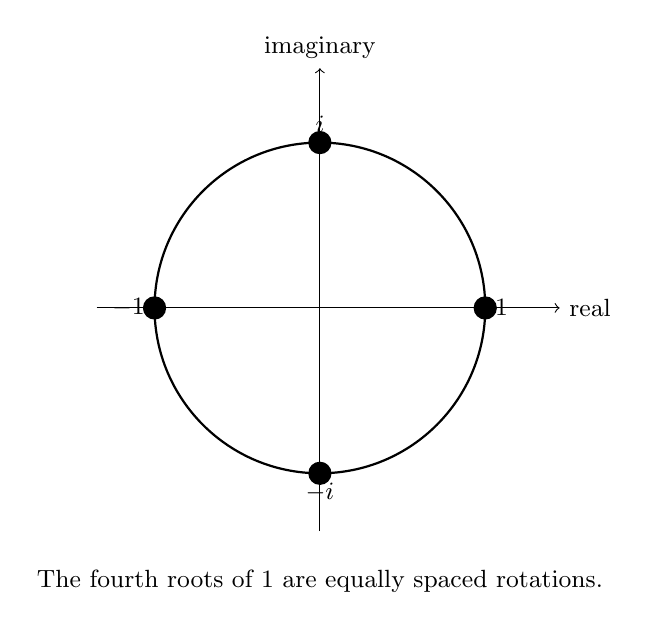
\begin{tikzpicture}[scale=2.1, every node/.style={font=\small}]
  \draw[->] (-1.35,0) -- (1.45,0) node[right] {real};
  \draw[->] (0,-1.35) -- (0,1.45) node[above] {imaginary};
  \draw[thick] (0,0) circle (1);

  \foreach \ang/\lab/\pos in {
    0/{1}/right,
    90/{i}/above,
    180/{-1}/left,
    270/{-i}/below} { % <-- Brace moved up, no comma
    \fill ({cos(\ang)},{sin(\ang)}) circle (2pt);
    \node[\pos] at ({cos(\ang)},{sin(\ang)}) {\(\lab\)};
  }

  \node at (0,-1.65) {The fourth roots of \(1\) are equally spaced rotations.};
\end{tikzpicture}
\caption{The equation \(z^4=1\) has four solutions on the unit circle.}
\label{fig:fourth-roots-unity}
\end{figure}

Euler's formula turns angle into exponent:

\[
e^{i\theta}e^{i\phi}
=
\bigl(\cos\theta+i\sin\theta\bigr)
\bigl(\cos\phi+i\sin\phi\bigr).
\]

By the multiplication rule in polar form,

\[
e^{i\theta}e^{i\phi}=e^{i(\theta+\phi)}.
\]

So multiplying unit complex numbers adds angles.  The exponential has become a
rotation machine.

\subsection{\texorpdfstring{Why \(e^{it}\) is the natural language of oscillation}{Why e^{it} is the natural language of oscillation}}
\label{subsec:eit-natural-language-oscillation}

Euler's formula says

\[
e^{it}=\cos t+i\sin t.
\]

As \(t\) changes, this complex number moves around the unit circle.

Its real part is

\[
\cos t,
\]

and its imaginary part is

\[
\sin t.
\]

So the moving point

\[
e^{it}
\]

is the same point we described parametrically earlier as

\[
(\cos t,\sin t).
\]

\begin{figure}[h]
\centering
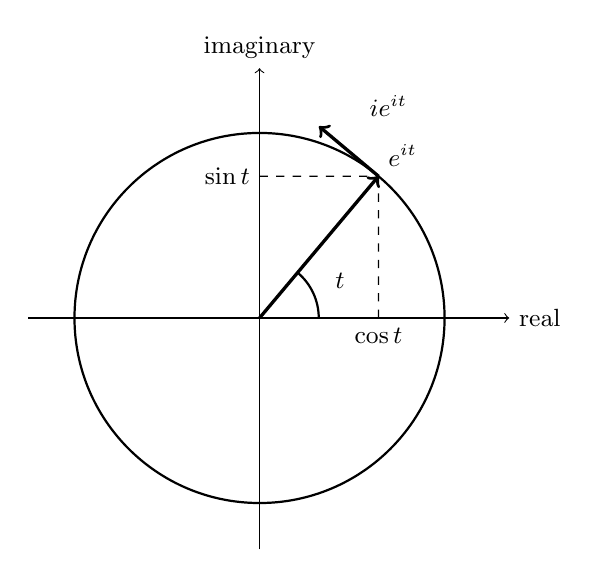
\begin{tikzpicture}[scale=2.35, every node/.style={font=\small}]
  \draw[->] (-1.25,0) -- (1.35,0) node[right] {real};
  \draw[->] (0,-1.25) -- (0,1.35) node[above] {imaginary};

  \draw[thick] (0,0) circle (1);

  \def\ang{50}
  \coordinate (P) at ({cos(\ang)},{sin(\ang)});
  \coordinate (V) at ({-sin(\ang)},{cos(\ang)});

  \draw[very thick,->] (0,0) -- (P);
  \draw[very thick,->] (P) -- ++({0.42*(-sin(\ang))},{0.42*cos(\ang)});

  \draw[dashed] ({cos(\ang)},0) -- (P);
  \draw[dashed] (0,{sin(\ang)}) -- (P);

  \draw[thick] (0.32,0) arc (0:\ang:0.32);

  \node at ({0.48*cos(25)},{0.48*sin(25)}) {\(t\)};
  \node[above right] at (P) {\(e^{it}\)};
  \node[right] at ({cos(\ang)-0.10},{sin(\ang)+0.38}) {\(ie^{it}\)};
  \node[below] at ({cos(\ang)},0) {\(\cos t\)};
  \node[left] at (0,{sin(\ang)}) {\(\sin t\)};
\end{tikzpicture}
\caption{The position \(e^{it}\) lies on the unit circle.  Its velocity \(ie^{it}\) is a quarter-turn of the position.}
\label{fig:eit-position-velocity}
\end{figure}

Differentiate the exponential series term by term, or use the exponential rule with the
chain rule:

\[
\boxed{
\frac{d}{dt}e^{it}=ie^{it}.
}
\]

Multiplication by \(i\) rotates by \(90^\circ\).  So the velocity of \(e^{it}\) is tangent to
the circle.

Differentiate again:

\[
\frac{d^2}{dt^2}e^{it}
=
i^2e^{it}
=
-e^{it}.
\]

Thus the acceleration points back toward the origin:

\[
\boxed{
\frac{d^2}{dt^2}e^{it}=-e^{it}.
}
\]

This is exactly the geometry of circular motion.

For angular frequency \(\omega>0\),

\[
e^{i\omega t}
=
\cos(\omega t)+i\sin(\omega t).
\]

Then

\[
\frac{d}{dt}e^{i\omega t}=i\omega e^{i\omega t},
\]

and

\[
\frac{d^2}{dt^2}e^{i\omega t}=-\omega^2 e^{i\omega t}.
\]

So

\[
\boxed{
z(t)=e^{i\omega t}
}
\]

solves the complex differential equation

\[
\boxed{
z''+\omega^2z=0.
}
\]

Taking real and imaginary parts gives

\[
\cos(\omega t)
\qquad\text{and}\qquad
\sin(\omega t),
\]

the two basic real oscillations.

More generally,

\[
A\cos(\omega t)+B\sin(\omega t)
\]

can be written as the real part of a complex exponential:

\[
\boxed{
A\cos(\omega t)+B\sin(\omega t)
=
\operatorname{Re}\bigl((A-Bi)e^{i\omega t}\bigr).
}
\]

The complex coefficient

\[
A-Bi
\]

stores the amplitude and phase.  The exponential

\[
e^{i\omega t}
\]

stores the rotation.

That is why complex numbers are not extra decoration.  They compress the language of
oscillation.

A vibrating spring is the next place this language becomes useful.

\section{Vibrations and second-order equations}
\label{sec:vibrations-second-order-equations}

Chapter \ref{chap:differential-equations} already introduced second-order equations
through vibrating systems.  A spring gave us

\[
y''+\omega^2y=0.
\]

At that time, sine and cosine solved the equation because their second derivatives return
negative copies of themselves.

Complex numbers explain the deeper reason:

\[
\text{oscillation is the shadow of rotation.}
\]

A point rotating in the complex plane has a horizontal shadow \(\cos(\omega t)\) and a
vertical shadow \(\sin(\omega t)\).  Those shadows move back and forth.  The spring
motion is one such shadow.

\subsection{The spring equation}
\label{subsec:spring-equation-ch17}

Picture a mass attached to a spring on a frictionless horizontal track.

Let

\[
y(t)=\text{displacement from equilibrium at time }t.
\]

The equilibrium position is

\[
y=0.
\]

Positive \(y\) means the mass is displaced to the right.  Negative \(y\) means the mass
is displaced to the left.

Hooke's law says that the spring force is proportional to displacement and points back
toward equilibrium:

\[
F_{\text{spring}}=-ky,
\qquad k>0.
\]

Newton's second law says

\[
F=ma.
\]

Here acceleration is the second derivative:

\[
a=y''.
\]

Thus

\[
my''=-ky.
\]

Rearrange:

\[
my''+ky=0.
\]

Divide by \(m\):

\[
y''+\frac{k}{m}y=0.
\]

It is customary to write

\[
\omega^2=\frac{k}{m},
\qquad \omega>0.
\]

Then the equation becomes

\[
\boxed{
y''+\omega^2y=0.
}
\]

This is the \emph{simple harmonic oscillator}.

\begin{figure}[h]
\centering
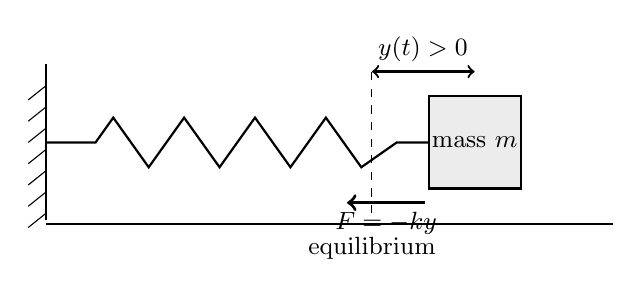
\begin{tikzpicture}[scale=0.9, every node/.style={font=\small}]
  % wall
  \draw[thick] (0,-1.1) -- (0,1.1);
  \foreach \y in {-1.0,-0.7,...,1.0} {
    \draw (0,\y) -- (-0.25,\y-0.2);
  }

  % track
  \draw[thick] (0,-1.15) -- (8,-1.15);

  % spring zigzag
  \draw[thick]
    (0,0) -- (0.7,0)
    -- (0.95,0.35)
    -- (1.45,-0.35)
    -- (1.95,0.35)
    -- (2.45,-0.35)
    -- (2.95,0.35)
    -- (3.45,-0.35)
    -- (3.95,0.35)
    -- (4.45,-0.35)
    -- (4.95,0)
    -- (5.4,0);

  % mass
  \draw[thick, fill=gray!15] (5.4,-0.65) rectangle (6.7,0.65);
  \node at (6.05,0) {mass \(m\)};

  % equilibrium dashed
  \draw[dashed] (4.6,-1.0) -- (4.6,1.0);
  \node[below] at (4.6,-1.2) {equilibrium};

  % displacement
  \draw[<->, thick] (4.6,1.0) -- (6.05,1.0);
  \node[above] at (5.32,1.0) {\(y(t)>0\)};

  % force arrow
  \draw[very thick,->] (5.35,-0.85) -- (4.25,-0.85);
  \node[below] at (4.8,-0.85) {\(F=-ky\)};
\end{tikzpicture}
\caption{A spring pulls back toward equilibrium.  Newton's law turns this restoring force into a second-order equation.}
\label{fig:spring-mass-equation}
\end{figure}

The equation says

\[
y''=-\omega^2y.
\]

So the acceleration always points opposite the displacement.  When the mass is to the
right, acceleration points left.  When the mass is to the left, acceleration points right.

That is what makes the motion reverse.

A second-order equation needs two initial conditions.  To know how the mass will move,
we need both its initial position and its initial velocity:

\[
y(0)=y_0,
\qquad
y'(0)=v_0.
\]

Position alone is not enough.  If the mass is at \(y=1\), it could be moving right, moving
left, or momentarily stopped.  Those motions have different futures.

\subsection{Sine and cosine as natural motions}
\label{subsec:sine-cosine-natural-motions}

The complex function

\[
z(t)=e^{i\omega t}
\]

satisfies

\[
z''+\omega^2z=0.
\]

Indeed,

\[
z'(t)=i\omega e^{i\omega t},
\]

and

\[
z''(t)=(i\omega)^2e^{i\omega t}
=
-\omega^2e^{i\omega t}.
\]

Therefore

\[
z''+\omega^2z=0.
\]

Now use Euler's formula:

\[
e^{i\omega t}=\cos(\omega t)+i\sin(\omega t).
\]

If

\[
z(t)=u(t)+iv(t),
\]

then

\[
z''+\omega^2z
=
\bigl(u''+\omega^2u\bigr)
+
i\bigl(v''+\omega^2v\bigr).
\]

For this complex expression to be \(0\), both real and imaginary parts must be \(0\).
So

\[
u''+\omega^2u=0,
\qquad
v''+\omega^2v=0.
\]

That means

\[
\cos(\omega t)
\qquad\text{and}\qquad
\sin(\omega t)
\]

are real solutions of

\[
y''+\omega^2y=0.
\]

Since the equation is linear, every linear combination is also a solution:

\[
\boxed{
y(t)=A\cos(\omega t)+B\sin(\omega t).
}
\]

This is the general real solution.

\begin{quote}
\textbf{Simple harmonic motion.}
The equation

\[
\boxed{
y''+\omega^2y=0,
\qquad \omega>0,
}
\]

has real solutions

\[
\boxed{
y(t)=A\cos(\omega t)+B\sin(\omega t).
}
\]

The constants \(A\) and \(B\) are determined by the initial position and initial velocity.
\end{quote}

Now impose

\[
y(0)=y_0,
\qquad
y'(0)=v_0.
\]

From

\[
y(t)=A\cos(\omega t)+B\sin(\omega t),
\]

we get

\[
y(0)=A.
\]

So

\[
A=y_0.
\]

Differentiate:

\[
y'(t)
=
-\omega A\sin(\omega t)+\omega B\cos(\omega t).
\]

Then

\[
y'(0)=\omega B.
\]

So

\[
B=\frac{v_0}{\omega}.
\]

Therefore

\[
\boxed{
y(t)=y_0\cos(\omega t)+\frac{v_0}{\omega}\sin(\omega t).
}
\]

\paragraph{Example.}
Solve

\[
y''+9y=0,
\qquad
y(0)=4,
\qquad
y'(0)=-6.
\]

Here

\[
\omega^2=9,
\qquad
\omega=3.
\]

So

\[
y(t)=A\cos(3t)+B\sin(3t).
\]

The initial position gives

\[
A=4.
\]

The initial velocity gives

\[
3B=-6,
\]

so

\[
B=-2.
\]

Thus

\[
\boxed{
y(t)=4\cos(3t)-2\sin(3t).
}
\]

The period is

\[
\boxed{
T=\frac{2\pi}{\omega}.
}
\]

Here

\[
T=\frac{2\pi}{3}.
\]

The solution repeats every \(2\pi/3\) units of time.

\paragraph{Amplitude and phase.}
Every expression of the form

\[
A\cos(\omega t)+B\sin(\omega t)
\]

can also be written as a shifted cosine:

\[
\boxed{
A\cos(\omega t)+B\sin(\omega t)=R\cos(\omega t-\phi),
}
\]

where

\[
R=\sqrt{A^2+B^2}.
\]

To see this, expand the right side:

\[
R\cos(\omega t-\phi)
=
R\cos(\omega t)\cos\phi+R\sin(\omega t)\sin\phi.
\]

So we need

\[
A=R\cos\phi,
\qquad
B=R\sin\phi.
\]

This is possible when

\[
R=\sqrt{A^2+B^2}.
\]

The number \(R\) is the \emph{amplitude}.  It is the largest distance from equilibrium.
The angle \(\phi\) is the \emph{phase shift}.  It tells where in the cycle the motion
starts.

For the example

\[
y(t)=4\cos(3t)-2\sin(3t),
\]

the amplitude is

\[
R=\sqrt{4^2+(-2)^2}=\sqrt{20}=2\sqrt5.
\]

The solution oscillates between

\[
-2\sqrt5
\qquad\text{and}\qquad
2\sqrt5.
\]

\begin{figure}[h]
\centering
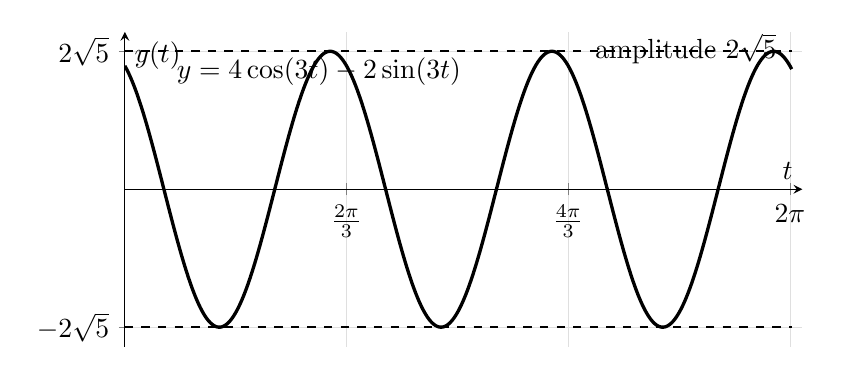
\begin{tikzpicture}
\begin{axis}[
    width=0.84\textwidth,
    height=0.46\textwidth,
    xmin=0, xmax=6.4,
    ymin=-5.1, ymax=5.1,
    axis lines=middle,
    xlabel={\(t\)},
    ylabel={\(y(t)\)},
    xtick={0,2.094,4.188,6.283},
    xticklabels={\(0\),\(\frac{2\pi}{3}\),\(\frac{4\pi}{3}\),\(2\pi\)},
    ytick={-4.472,0,4.472},
    yticklabels={\(-2\sqrt5\),\(0\),\(2\sqrt5\)},
    grid=both,
    grid style={line width=.1pt, draw=gray!25},
]
\addplot[very thick, domain=0:6.3, samples=400] {4*cos(deg(3*x))-2*sin(deg(3*x))};
\addplot[thick, dashed, domain=0:6.3, samples=2] {sqrt(20)};
\addplot[thick, dashed, domain=0:6.3, samples=2] {-sqrt(20)};
\node[anchor=west] at (axis cs:0.4,3.8) {\(y=4\cos(3t)-2\sin(3t)\)};
\node[anchor=west] at (axis cs:4.35,4.55) {amplitude \(2\sqrt5\)};
\end{axis}
\end{tikzpicture}
\caption{The solution of \(y''+9y=0\) is periodic.  Its amplitude is determined by the initial position and velocity.}
\label{fig:spring-solution-amplitude-phase}
\end{figure}

The complex form stores this same information in one coefficient:

\[
A\cos(\omega t)+B\sin(\omega t)
=
\operatorname{Re}\bigl((A-Bi)e^{i\omega t}\bigr).
\]

The modulus

\[
|A-Bi|=\sqrt{A^2+B^2}
\]

is the amplitude.  The argument gives the phase.

This is the compact power of complex notation: amplitude and phase become length and
angle.

\subsection{Energy conservation}
\label{subsec:energy-conservation-spring}

The spring equation also contains a conservation law.

Return to the physical form

\[
my''+ky=0.
\]

The kinetic energy is

\[
\frac12m(y')^2,
\]

and the spring potential energy is

\[
\frac12ky^2.
\]

Define the total energy

\[
\boxed{
E(t)=\frac12m\bigl(y'(t)\bigr)^2+\frac12k\bigl(y(t)\bigr)^2.
}
\]

Differentiate:

\[
E'(t)
=
m y'(t)y''(t)+k y(t)y'(t).
\]

Factor \(y'(t)\):

\[
E'(t)
=
y'(t)\bigl(my''(t)+ky(t)\bigr).
\]

But the spring equation says

\[
my''+ky=0.
\]

Therefore

\[
\boxed{
E'(t)=0.
}
\]

So

\[
\boxed{
E(t)\text{ is constant.}
}
\]

This is the calculus meaning of conservation:

\[
\boxed{
\text{a conserved quantity is a quantity whose derivative is zero.}
}
\]

The Mean Value Theorem then tells us that the quantity is constant on the interval.

\paragraph{Interpretation.}
At a turning point, the mass is momentarily stopped:

\[
y'=0.
\]

So all the energy is spring potential energy:

\[
E=\frac12ky^2.
\]

At equilibrium,

\[
y=0,
\]

so all the energy is kinetic energy:

\[
E=\frac12m(y')^2.
\]

The energy does not disappear.  It changes form.

\paragraph{Energy ellipse.}
For the solution

\[
y(t)=R\cos(\omega t),
\qquad
\omega^2=\frac{k}{m},
\]

the velocity is

\[
y'(t)=-R\omega\sin(\omega t).
\]

Then

\[
\frac{y^2}{R^2}+\frac{(y')^2}{\omega^2R^2}
=
\cos^2(\omega t)+\sin^2(\omega t)
=
1.
\]

So in the phase plane, whose coordinates are

\[
(y,y'),
\]

the motion follows an ellipse:

\[
\boxed{
\frac{y^2}{R^2}+\frac{(y')^2}{\omega^2R^2}=1.
}
\]

\begin{figure}[h]
\centering
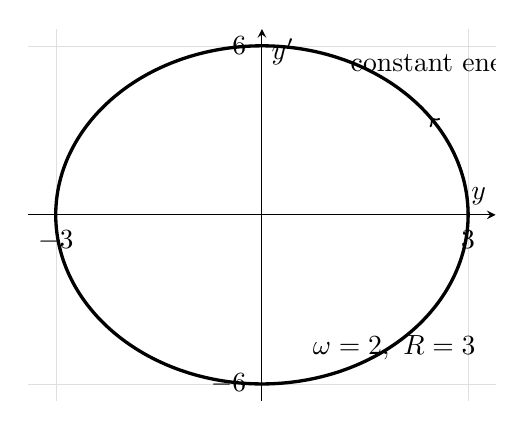
\begin{tikzpicture}
\begin{axis}[
    width=0.62\textwidth,
    height=0.52\textwidth,
    xmin=-3.4, xmax=3.4,
    ymin=-6.6, ymax=6.6,
    axis lines=middle,
    xlabel={\(y\)},
    ylabel={\(y'\)},
    xtick={-3,0,3},
    ytick={-6,0,6},
    grid=both,
    grid style={line width=.1pt, draw=gray!25},
]
\addplot[very thick, domain=0:360, samples=300] ({3*cos(x)},{6*sin(x)});
\draw[->, thick] (axis cs:3,0) arc [start angle=0, end angle=35, x radius=3, y radius=6];
\node[anchor=west] at (axis cs:1.15,5.3) {constant energy curve};
\node[anchor=west] at (axis cs:0.6,-4.7) {\(\omega=2,\ R=3\)};
\end{axis}
\end{tikzpicture}
\caption{For an undamped oscillator, the phase point \((y,y')\) moves around a closed energy curve.}
\label{fig:phase-plane-energy-ellipse}
\end{figure}

This picture gives another way to see why the motion repeats.  The phase point moves
around a closed curve instead of spiraling inward or escaping outward.

The conserved energy is what keeps it there.

\subsection{Damping and forcing preview}
\label{subsec:damping-forcing-preview}

Real oscillations rarely continue forever.  A guitar string fades.  A swing slows down.
A car's suspension settles after a bump.

A damping force resists velocity.  A simple model is

\[
F_{\text{damping}}=-cy',
\qquad c>0.
\]

The spring force is still

\[
F_{\text{spring}}=-ky.
\]

Newton's law gives

\[
my''=-cy'-ky.
\]

So the damped spring equation is

\[
\boxed{
my''+cy'+ky=0.
}
\]

Use the same energy as before:

\[
E(t)=\frac12m(y')^2+\frac12ky^2.
\]

Then

\[
E'(t)=y'(my''+ky).
\]

From the damped equation,

\[
my''+ky=-cy'.
\]

Therefore

\[
\boxed{
E'(t)=-c(y')^2\le0.
}
\]

The energy decreases.  The damping term drains energy from the system.

\begin{quote}
\textbf{Damping.}
In the model

\[
my''+cy'+ky=0,
\]

the term \(cy'\) removes energy.  If \(c>0\), then

\[
E'(t)=-c(y')^2\le0.
\]
\end{quote}

Complex numbers also help describe the shape of damped motion.

Try a solution of the form

\[
y=e^{\lambda t}.
\]

Substituting into

\[
my''+cy'+ky=0
\]

gives

\[
m\lambda^2e^{\lambda t}+c\lambda e^{\lambda t}+ke^{\lambda t}=0.
\]

Since \(e^{\lambda t}\neq0\), we need

\[
\boxed{
m\lambda^2+c\lambda+k=0.
}
\]

This is called the \emph{characteristic equation}.

When damping is light,

\[
c^2<4mk,
\]

the roots are complex:

\[
\lambda
=
-\frac{c}{2m}\pm i\mu,
\]

where

\[
\mu=\sqrt{\frac{k}{m}-\left(\frac{c}{2m}\right)^2}.
\]

The solutions have the form

\[
\boxed{
y(t)=e^{-ct/(2m)}
\bigl(A\cos(\mu t)+B\sin(\mu t)\bigr).
}
\]

The sine and cosine still oscillate.  The exponential factor

\[
e^{-ct/(2m)}
\]

shrinks the amplitude.

\begin{figure}[h]
\centering
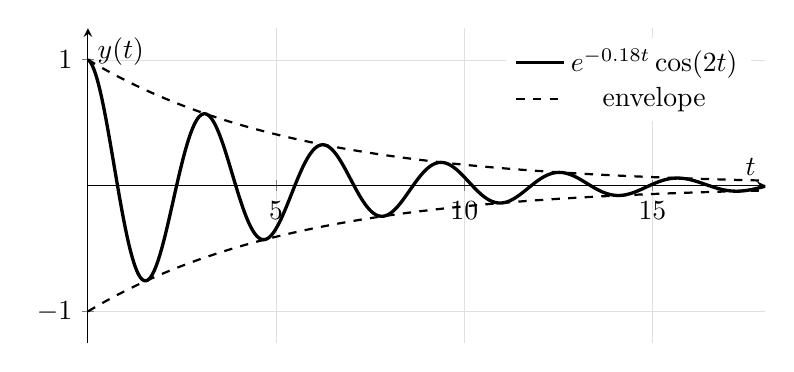
\begin{tikzpicture}
\begin{axis}[
    width=0.84\textwidth,
    height=0.46\textwidth,
    xmin=0, xmax=18,
    ymin=-1.25, ymax=1.25,
    axis lines=middle,
    xlabel={\(t\)},
    ylabel={\(y(t)\)},
    xtick={0,5,10,15},
    ytick={-1,0,1},
    grid=both,
    grid style={line width=.1pt, draw=gray!25},
    legend style={draw=none, at={(0.98,0.97)}, anchor=north east}
]
\addplot[very thick, domain=0:18, samples=500] {exp(-0.18*x)*cos(deg(2*x))};
\addlegendentry{\(e^{-0.18t}\cos(2t)\)}
\addplot[thick, dashed, domain=0:18, samples=200] {exp(-0.18*x)};
\addlegendentry{envelope}
\addplot[thick, dashed, domain=0:18, samples=200] {-exp(-0.18*x)};
\end{axis}
\end{tikzpicture}
\caption{A lightly damped oscillator still oscillates, but its amplitude shrinks exponentially.}
\label{fig:chapter17-damped-oscillation}
\end{figure}

Now add an outside force.  A child pushes a swing.  A motor shakes a machine.  Wind
pushes a bridge.  A simple periodically forced model is

\[
\boxed{
my''+cy'+ky=F_0\cos(\gamma t).
}
\]

The number \(\gamma\) is the driving angular frequency.

Complex notation lets us replace the cosine forcing by the real part of

\[
F_0e^{i\gamma t}.
\]

Look for a complex steady-state response

\[
z(t)=Ce^{i\gamma t}.
\]

Then

\[
z'=i\gamma Ce^{i\gamma t},
\]

and

\[
z''=-\gamma^2Ce^{i\gamma t}.
\]

Substitute into

\[
mz''+cz'+kz=F_0e^{i\gamma t}.
\]

We get

\[
\bigl(-m\gamma^2+i c\gamma+k\bigr)Ce^{i\gamma t}
=
F_0e^{i\gamma t}.
\]

Cancel \(e^{i\gamma t}\):

\[
\bigl(k-m\gamma^2+i c\gamma\bigr)C=F_0.
\]

Thus

\[
\boxed{
C=\frac{F_0}{k-m\gamma^2+i c\gamma}.
}
\]

The real part of

\[
Ce^{i\gamma t}
\]

gives the physical steady-state motion.

The amplitude of the steady-state response is the modulus of \(C\):

\[
\boxed{
|C|
=
\frac{F_0}
{\sqrt{(k-m\gamma^2)^2+(c\gamma)^2}}.
}
\]

This formula explains resonance with damping.  The response is large when

\[
k-m\gamma^2
\]

is small, meaning the driving frequency is near the natural frequency.  But if \(c>0\),
the denominator never becomes \(0\), because of the term

\[
(c\gamma)^2.
\]

Damping prevents infinite growth in this simple steady-state model.

\begin{figure}[h]
\centering
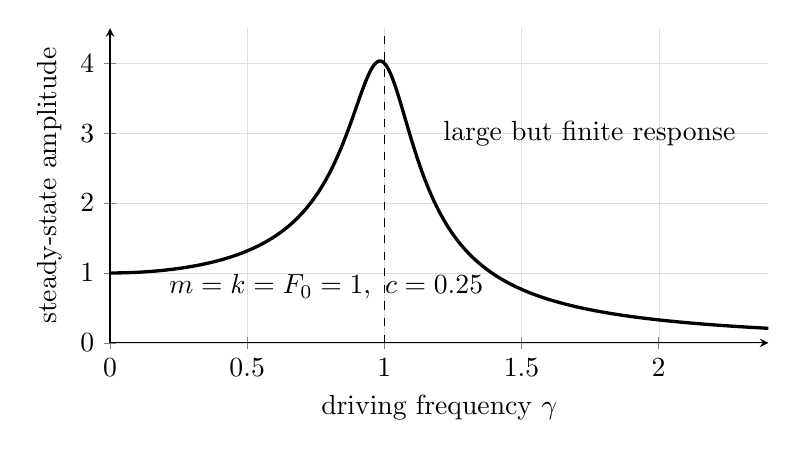
\begin{tikzpicture}
\begin{axis}[
    width=0.82\textwidth,
    height=0.46\textwidth,
    xmin=0, xmax=2.4,
    ymin=0, ymax=4.5,
    axis lines=left,
    xlabel={driving frequency \(\gamma\)},
    ylabel={steady-state amplitude},
    xtick={0,0.5,1,1.5,2},
    ytick={0,1,2,3,4},
    grid=both,
    grid style={line width=.1pt, draw=gray!25},
]
\addplot[very thick, domain=0:2.4, samples=400] {1/sqrt((1-x^2)^2+(0.25*x)^2)};
\draw[dashed] (axis cs:1,0) -- (axis cs:1,4.5);
\node[anchor=south] at (axis cs:1,4.5) {near natural frequency};
\node[anchor=west] at (axis cs:1.18,3.0) {large but finite response};
\node[anchor=west] at (axis cs:0.18,0.8) {\(m=k=F_0=1,\ c=0.25\)};
\end{axis}
\end{tikzpicture}
\caption{With damping, resonance produces a large response near the natural frequency, but the amplitude remains finite.}
\label{fig:damped-forced-response}
\end{figure}

The formula is more advanced than the rest of this book, but the idea is not advanced:

\[
\boxed{
\text{periodic input} \quad\Longrightarrow\quad \text{periodic response}.
}
\]

Complex numbers make the calculation shorter because they carry amplitude and phase
together.

A single vibrating spring is one wave.  Many sounds, signals, and periodic motions are
built from many waves at once.  The next question is the beginning of Fourier's idea:

\[
\text{Can complicated periodic motion be built from sines and cosines?}
\]

\section{Fourier series preview}
\label{sec:fourier-series-preview}

A single spring gives one clean frequency:

\[
\cos(\omega t)
\qquad\text{or}\qquad
\sin(\omega t).
\]

But real periodic motion is rarely one pure wave.  A violin string, an electrical signal,
a heartbeat, a tide table, and a repeating temperature pattern all contain mixtures.

Taylor series built functions from powers:

\[
1,\ x,\ x^2,\ x^3,\ldots.
\]

Fourier series build periodic functions from waves:

\[
1,\ \cos t,\ \sin t,\ \cos(2t),\ \sin(2t),\ \cos(3t),\ \sin(3t),\ldots.
\]

This section is a preview.  The full convergence theory belongs to a later course.  But
the main idea is already visible with the calculus we know:

\[
\boxed{
\text{Fourier series use integrals to measure how much of each wave is present.}
}
\]

\subsection{Building a periodic function from waves}
\label{subsec:building-periodic-function-from-waves}

A function \(f\) is \emph{periodic} with period \(2\pi\) if

\[
f(t+2\pi)=f(t)
\]

for every \(t\).

The basic waves

\[
\cos(nt)
\qquad\text{and}\qquad
\sin(nt)
\]

are all \(2\pi\)-periodic when \(n\) is a positive integer.  The integer \(n\) counts how
many full oscillations occur during one interval of length \(2\pi\).

A finite mixture of these waves has the form

\[
P_N(t)
=
\frac{a_0}{2}
+
\sum_{n=1}^{N}
\bigl(a_n\cos(nt)+b_n\sin(nt)\bigr).
\]

This is called a \emph{trigonometric polynomial}.  It is a finite Fourier approximation.

\begin{quote}
\textbf{Fourier idea.}
For a \(2\pi\)-periodic function \(f\), try to write

\[
\boxed{
f(t)
\sim
\frac{a_0}{2}
+
\sum_{n=1}^{\infty}
\bigl(a_n\cos(nt)+b_n\sin(nt)\bigr).
}
\]

The coefficients \(a_n\) and \(b_n\) measure how much of each cosine and sine wave is
present.
\end{quote}

The symbol

\[
\sim
\]

is being used carefully.  It means ``has Fourier series.''  It does not automatically mean
that the series converges everywhere to \(f(t)\).  Convergence is part of the deeper
theory.

Still, the guiding picture is simple:

\[
\boxed{
\text{complicated periodic motion can often be approximated by adding simple waves.}
}
\]

\begin{figure}[h]
\centering
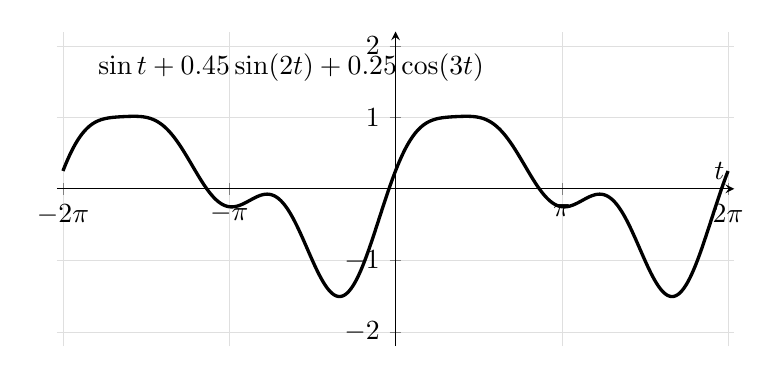
\begin{tikzpicture}
\begin{axis}[
    width=0.84\textwidth,
    height=0.46\textwidth,
    xmin=-6.4, xmax=6.4,
    ymin=-2.2, ymax=2.2,
    axis lines=middle,
    xlabel={\(t\)},
    ylabel={},
    xtick={-6.283,-3.1416,0,3.1416,6.283},
    xticklabels={\(-2\pi\),\(-\pi\),\(0\),\(\pi\),\(2\pi\)},
    ytick={-2,-1,0,1,2},
    grid=both,
    grid style={line width=.1pt, draw=gray!25},
]
\addplot[very thick, domain=-6.283:6.283, samples=600]
  {sin(deg(x)) + 0.45*sin(deg(2*x)) + 0.25*cos(deg(3*x))};
\node[anchor=west] at (axis cs:-5.8,1.7)
  {\(\sin t+0.45\sin(2t)+0.25\cos(3t)\)};
\end{axis}
\end{tikzpicture}
\caption{Adding a few sine and cosine waves already creates a more complicated periodic shape.}
\label{fig:fourier-wave-mixture}
\end{figure}

This is why Fourier series belong after vibrations.  One oscillator gives one wave.
Many oscillators, or one complicated periodic signal, give a mixture.

\subsection{Orthogonality of sine and cosine, geometrically}
\label{subsec:orthogonality-sine-cosine-geometrically}

To find the coefficients in a Fourier series, we need a way to measure how much one
function points in the direction of another.

For ordinary vectors, the dot product measures alignment.  Perpendicular vectors have
dot product zero.

For functions on \([-\pi,\pi]\), the analogous dot product is an integral:

\[
\boxed{
\langle f,g\rangle
=
\int_{-\pi}^{\pi} f(t)g(t)\,dt.
}
\]

If

\[
\langle f,g\rangle=0,
\]

we say the functions are \emph{orthogonal} on \([-\pi,\pi]\).

This language is geometric.  The functions are being treated like vectors, but with
infinitely many coordinates.

\paragraph{Example.}
The functions \(\sin t\) and \(\sin(2t)\) are orthogonal on \([-\pi,\pi]\), because

\[
\int_{-\pi}^{\pi} \sin t\sin(2t)\,dt=0.
\]

Use the product-to-sum identity

\[
\sin A\sin B
=
\frac12\bigl(\cos(A-B)-\cos(A+B)\bigr).
\]

With \(A=t\) and \(B=2t\),

\[
\sin t\sin(2t)
=
\frac12\bigl(\cos t-\cos(3t)\bigr).
\]

Therefore

\[
\int_{-\pi}^{\pi}\sin t\sin(2t)\,dt
=
\frac12\int_{-\pi}^{\pi}\cos t\,dt
-
\frac12\int_{-\pi}^{\pi}\cos(3t)\,dt.
\]

Both integrals are zero over a full symmetric period.  Hence

\[
\boxed{
\int_{-\pi}^{\pi}\sin t\sin(2t)\,dt=0.
}
\]

\begin{figure}[h]
\centering
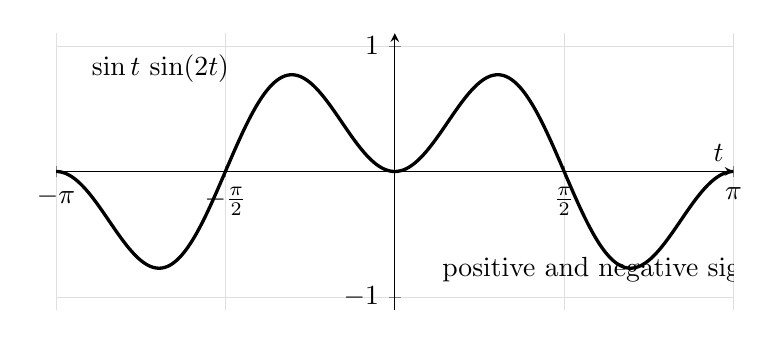
\begin{tikzpicture}
\begin{axis}[
    width=0.84\textwidth,
    height=0.42\textwidth,
    xmin=-3.1416, xmax=3.1416,
    ymin=-1.1, ymax=1.1,
    axis lines=middle,
    xlabel={\(t\)},
    ylabel={},
    xtick={-3.1416,-1.5708,0,1.5708,3.1416},
    xticklabels={\(-\pi\),\(-\frac{\pi}{2}\),\(0\),\(\frac{\pi}{2}\),\(\pi\)},
    ytick={-1,0,1},
    grid=both,
    grid style={line width=.1pt, draw=gray!25},
]
\addplot[very thick, domain=-3.1416:3.1416, samples=500]
  {sin(deg(x))*sin(deg(2*x))};
\node[anchor=west] at (axis cs:-2.9,0.82)
  {\(\sin t\,\sin(2t)\)};
\node[anchor=west] at (axis cs:0.35,-0.78)
  {positive and negative signed areas cancel};
\end{axis}
\end{tikzpicture}
\caption{The product \(\sin t\sin(2t)\) has signed area zero over \([-\pi,\pi]\).}
\label{fig:orthogonality-product-signed-area}
\end{figure}

The same cancellation happens systematically.  If \(m\) and \(n\) are positive integers,
then

\[
\int_{-\pi}^{\pi}\cos(mt)\cos(nt)\,dt=0
\qquad\text{when }m\neq n,
\]

\[
\int_{-\pi}^{\pi}\sin(mt)\sin(nt)\,dt=0
\qquad\text{when }m\neq n,
\]

and

\[
\int_{-\pi}^{\pi}\sin(mt)\cos(nt)\,dt=0
\]

for all \(m,n\).

The only time a sine or cosine wave has nonzero dot product with itself is when the
frequencies match:

\[
\int_{-\pi}^{\pi}\cos^2(nt)\,dt=\pi,
\qquad n\ge1,
\]

\[
\int_{-\pi}^{\pi}\sin^2(nt)\,dt=\pi,
\qquad n\ge1.
\]

Also,

\[
\int_{-\pi}^{\pi}1^2\,dt=2\pi.
\]

These facts are the engine of Fourier coefficients.

Suppose, at least formally, that

\[
f(t)
\sim
\frac{a_0}{2}
+
\sum_{n=1}^{\infty}
\bigl(a_n\cos(nt)+b_n\sin(nt)\bigr).
\]

Multiply both sides by \(\cos(mt)\) and integrate from \(-\pi\) to \(\pi\).  Orthogonality
kills every term except the matching cosine term:

\[
\int_{-\pi}^{\pi} f(t)\cos(mt)\,dt
=
a_m\int_{-\pi}^{\pi}\cos^2(mt)\,dt
=
a_m\pi.
\]

So

\[
\boxed{
a_m=
\frac1\pi
\int_{-\pi}^{\pi} f(t)\cos(mt)\,dt,
\qquad m\ge1.
}
\]

Similarly,

\[
\boxed{
b_m=
\frac1\pi
\int_{-\pi}^{\pi} f(t)\sin(mt)\,dt,
\qquad m\ge1.
}
\]

For the constant term,

\[
\int_{-\pi}^{\pi} f(t)\,dt
=
\int_{-\pi}^{\pi}\frac{a_0}{2}\,dt
=
a_0\pi.
\]

Thus

\[
\boxed{
a_0=
\frac1\pi
\int_{-\pi}^{\pi} f(t)\,dt.
}
\]

\begin{quote}
\textbf{Fourier coefficients on \([-\pi,\pi]\).}
For a \(2\pi\)-periodic function \(f\), the Fourier coefficients are

\[
\boxed{
a_0=
\frac1\pi
\int_{-\pi}^{\pi} f(t)\,dt,
}
\]

\[
\boxed{
a_n=
\frac1\pi
\int_{-\pi}^{\pi} f(t)\cos(nt)\,dt,
\qquad n\ge1,
}
\]

and

\[
\boxed{
b_n=
\frac1\pi
\int_{-\pi}^{\pi} f(t)\sin(nt)\,dt,
\qquad n\ge1.
}
\]
\end{quote}

The formulas use integrals because integrals are dot products for functions.

For finite trigonometric polynomials, this derivation is exact.  For infinite Fourier
series, one must justify the limiting step.  That is part of Fourier analysis.  The preview
idea remains:

\[
\boxed{
\text{integrate against a wave to measure the amount of that wave.}
}
\]

\subsection{Square waves and Gibbs phenomenon}
\label{subsec:square-waves-gibbs-phenomenon}

Fourier's idea becomes surprising when the target function has corners or jumps.

Consider the \(2\pi\)-periodic square wave

\[
Q(t)=
\begin{cases}
-1, & -\pi<t<0,\\
1, & 0<t<\pi.
\end{cases}
\]

Then repeat this pattern with period \(2\pi\).  The values at the jump points can be
assigned separately; they do not change the integrals that determine the coefficients.

This function is odd:

\[
Q(-t)=-Q(t).
\]

Cosine is even, so

\[
Q(t)\cos(nt)
\]

is odd.  The integral of an odd function over \([-\pi,\pi]\) is zero.  Therefore all cosine
coefficients are zero:

\[
a_n=0.
\]

Also,

\[
a_0=0.
\]

Only sine terms remain.

For \(n\ge1\),

\[
b_n=
\frac1\pi
\int_{-\pi}^{\pi} Q(t)\sin(nt)\,dt.
\]

Since \(Q(t)\sin(nt)\) is even,

\[
b_n=
\frac2\pi
\int_0^\pi \sin(nt)\,dt.
\]

Compute:

\[
\int_0^\pi \sin(nt)\,dt
=
\left[-\frac{\cos(nt)}{n}\right]_0^\pi
=
\frac{1-\cos(n\pi)}{n}.
\]

Since

\[
\cos(n\pi)=(-1)^n,
\]

we get

\[
b_n=
\frac2\pi
\cdot
\frac{1-(-1)^n}{n}.
\]

If \(n\) is even, then \((-1)^n=1\), so

\[
b_n=0.
\]

If \(n\) is odd, then \((-1)^n=-1\), so

\[
b_n=\frac{4}{\pi n}.
\]

Therefore the square wave has Fourier series

\[
\boxed{
Q(t)
\sim
\frac4\pi
\left(
\sin t+\frac{\sin(3t)}{3}
+\frac{\sin(5t)}{5}
+\frac{\sin(7t)}{7}
+\cdots
\right).
}
\]

The \(N\)-th odd partial sum is

\[
\boxed{
S_N(t)
=
\frac4\pi
\sum_{k=0}^{N}
\frac{\sin((2k+1)t)}{2k+1}.
}
\]

\begin{figure}[h]
\centering
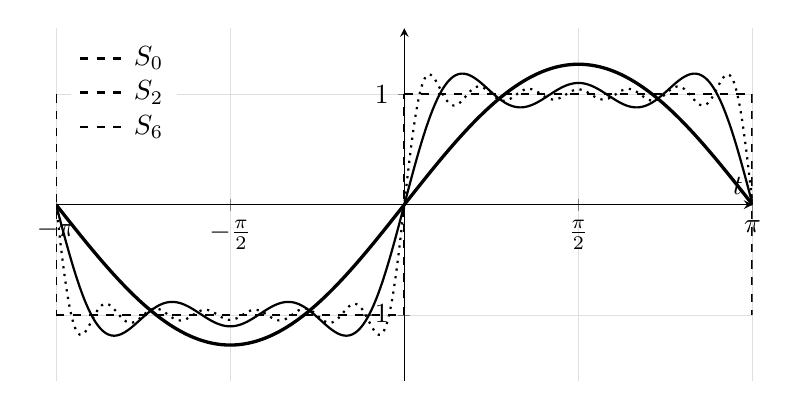
\begin{tikzpicture}
\begin{axis}[
    width=0.86\textwidth,
    height=0.50\textwidth,
    xmin=-3.1416, xmax=3.1416,
    ymin=-1.6, ymax=1.6,
    axis lines=middle,
    xlabel={\(t\)},
    ylabel={},
    xtick={-3.1416,-1.5708,0,1.5708,3.1416},
    xticklabels={\(-\pi\),\(-\frac{\pi}{2}\),\(0\),\(\frac{\pi}{2}\),\(\pi\)},
    ytick={-1,0,1},
    grid=both,
    grid style={line width=.1pt, draw=gray!25},
    legend style={draw=none, at={(0.02,0.98)}, anchor=north west}
]
% square wave
\addplot[thick, dashed, domain=-3.1416:0, samples=2] {-1};
\addplot[thick, dashed, domain=0:3.1416, samples=2] {1};
\addplot[thick, dashed] coordinates {(-3.1416,1) (-3.1416,-1)};
\addplot[thick, dashed] coordinates {(0,-1) (0,1)};
\addplot[thick, dashed] coordinates {(3.1416,1) (3.1416,-1)};

% partial sums
\addplot[very thick, domain=-3.1416:3.1416, samples=900]
  {4/3.14159*(sin(deg(x)))};
\addlegendentry{\(S_0\)}
\addplot[thick, domain=-3.1416:3.1416, samples=900]
  {4/3.14159*(sin(deg(x)) + sin(deg(3*x))/3 + sin(deg(5*x))/5)};
\addlegendentry{\(S_2\)}
\addplot[thick, dotted, domain=-3.1416:3.1416, samples=900]
  {4/3.14159*(sin(deg(x)) + sin(deg(3*x))/3 + sin(deg(5*x))/5 + sin(deg(7*x))/7 + sin(deg(9*x))/9 + sin(deg(11*x))/11 + sin(deg(13*x))/13)};
\addlegendentry{\(S_6\)}
\end{axis}
\end{tikzpicture}
\caption{Fourier partial sums approximate a square wave by adding sine waves.  Near each jump, ripples remain.}
\label{fig:square-wave-fourier-partial-sums}
\end{figure}

The approximation improves away from the jumps.  But near a jump, something strange
happens.  The partial sums overshoot the top level and undershoot the bottom level.

As we add more terms, the ripples get narrower.  But the first overshoot near the jump
does not simply disappear.  It approaches a persistent limiting size.

This is called the \emph{Gibbs phenomenon}.

\begin{quote}
\textbf{Gibbs phenomenon.}
Fourier partial sums of a function with a jump often overshoot near the jump.  Adding
more terms makes the overshoot region narrower, but the overshoot height approaches
a persistent limiting size.
\end{quote}

There is also a convergence warning at the jump itself.  The square wave jumps from
\(-1\) to \(1\) at \(t=0\).  The Fourier series does not choose the left value or the right
value.  It converges to the midpoint:

\[
\frac{-1+1}{2}=0.
\]

More generally, for a sufficiently well-behaved periodic function, the Fourier series
converges at a jump to the average of the left-hand and right-hand limits.

That is a new kind of honesty.  Fourier series can represent discontinuous shapes, but
they do not erase the discontinuity.  The jump leaves a visible trace in the approximation.

\subsection{Why Fourier series belong after Taylor series}
\label{subsec:why-fourier-after-taylor}

Taylor series and Fourier series are cousins.  Both try to build complicated functions
from simple functions.

But they have different personalities.

\begin{center}
\renewcommand{\arraystretch}{1.35}
\begin{tabular}{c|c|c}
\textbf{series type} & \textbf{building blocks} & \textbf{main viewpoint} \\ \hline
Taylor series &
\(1,(x-a),(x-a)^2,(x-a)^3,\ldots\) &
local behavior near a center \(a\) \\

Fourier series &
\(1,\cos t,\sin t,\cos(2t),\sin(2t),\ldots\) &
periodic behavior over a whole cycle
\end{tabular}
\end{center}

A Taylor series asks:

\[
\text{How does the function behave near one point?}
\]

A Fourier series asks:

\[
\text{What frequencies make up this repeating shape?}
\]

Taylor coefficients come from derivatives at one point:

\[
f(a),\quad f'(a),\quad f''(a),\quad \ldots.
\]

Fourier coefficients come from integrals over a whole period:

\[
\int_{-\pi}^{\pi} f(t)\cos(nt)\,dt,
\qquad
\int_{-\pi}^{\pi} f(t)\sin(nt)\,dt.
\]

So Taylor series are local.  Fourier series are global over a period.

This also explains why Fourier series can handle jumps better than Taylor series.  A
Taylor series is tied to local differentiability at a center.  A Fourier series is built from
waves and measures average alignment over an interval.  It can still make sense when
the function has corners or jumps.

Euler's formula compresses the real waves into complex exponentials:

\[
e^{int}=\cos(nt)+i\sin(nt).
\]

So a Fourier series can also be written in the compact complex form

\[
\boxed{
f(t)\sim\sum_{n=-\infty}^{\infty} c_n e^{int}.
}
\]

The corresponding coefficients are

\[
\boxed{
c_n=
\frac{1}{2\pi}
\int_{-\pi}^{\pi} f(t)e^{-int}\,dt.
}
\]

This form belongs more naturally to a later course, but the meaning is already visible:

\[
\boxed{
\text{complex exponentials are rotating waves, and Fourier series add rotating waves.}
}
\]

The chapter began with a rotating exponential, reached vibrating springs, and then
combined many waves.  One more bridge remains.  The Fundamental Theorem of
Calculus was the hinge of single-variable calculus.  It also has a second life: it is the
first example of a boundary theorem.

\section{The one-dimensional Stokes theorem}
\label{sec:one-dimensional-stokes-theorem}

The Fundamental Theorem told us that

\[
\int_a^b F'(x)\,dx=F(b)-F(a).
\]

At first, this was an antiderivative rule.  It let us evaluate integrals.  But there is a
deeper geometric reading:

\[
\boxed{
\text{what accumulates inside an interval is measured by what happens on its boundary.}
}
\]

In one dimension, the boundary of an interval consists of two endpoints.  The right
endpoint counts positively.  The left endpoint counts negatively.

That signed boundary is the seed of Stokes' theorem.

\subsection{Boundary of an interval}
\label{subsec:boundary-of-interval}

An interval is not just a set of points.  When we write

\[
\int_a^b f(x)\,dx,
\]

we are traveling from \(a\) to \(b\).  The direction matters.  Reversing the direction
changes the sign:

\[
\int_b^a f(x)\,dx=-\int_a^b f(x)\,dx.
\]

So the oriented interval from \(a\) to \(b\) has an oriented boundary.

\[
\boxed{
\partial[a,b]=\{b\}-\{a\}.
}
\]

This notation says:

\[
\text{right endpoint} \quad - \quad \text{left endpoint}.
\]

The endpoint \(b\) has sign \(+\).  The endpoint \(a\) has sign \(-\).

\begin{figure}[h]
\centering
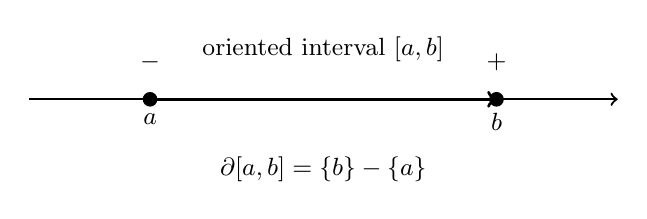
\begin{tikzpicture}[scale=1.1, every node/.style={font=\small}]
  \draw[->, thick] (-0.4,0) -- (6.4,0);
  \draw[very thick, ->] (1,0) -- (5,0);

  \fill (1,0) circle (2.4pt);
  \fill (5,0) circle (2.4pt);

  \node[below] at (1,-0.05) {\(a\)};
  \node[below] at (5,-0.05) {\(b\)};

  \node[above] at (1,0.22) {\(-\)};
  \node[above] at (5,0.22) {\(+\)};

  \node[above] at (3,0.32) {oriented interval \([a,b]\)};
  \node[below] at (3,-0.55) {\(\partial[a,b]=\{b\}-\{a\}\)};
\end{tikzpicture}
\caption{The boundary of an oriented interval is its ending point minus its starting point.}
\label{fig:oriented-interval-boundary}
\end{figure}

This sign convention is not decoration.  It is what makes intervals add correctly.

Suppose

\[
a<c<b.
\]

Then the interval \([a,b]\) can be split into

\[
[a,c]
\qquad\text{and}\qquad
[c,b].
\]

Their boundaries are

\[
\partial[a,c]=\{c\}-\{a\},
\]

and

\[
\partial[c,b]=\{b\}-\{c\}.
\]

Add them:

\[
\bigl(\{c\}-\{a\}\bigr)+\bigl(\{b\}-\{c\}\bigr)=\{b\}-\{a\}.
\]

The interior point \(c\) cancels.

\[
\boxed{
\text{interior boundaries cancel; only the outer boundary remains.}
}
\]

\begin{figure}[h]
\centering
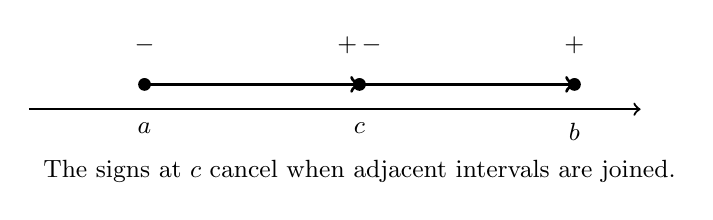
\begin{tikzpicture}[scale=1.05, every node/.style={font=\small}]
  \draw[->, thick] (-0.4,0) -- (7.0,0);

  \draw[very thick, ->] (1,0.3) -- (3.6,0.3);
  \draw[very thick, ->] (3.6,0.3) -- (6.2,0.3);

  \fill (1,0.3) circle (2.2pt);
  \fill (3.6,0.3) circle (2.2pt);
  \fill (6.2,0.3) circle (2.2pt);

  \node[above] at (1,0.55) {\(-\)};
  \node[above] at (3.6,0.55) {\(+\,-\)};
  \node[above] at (6.2,0.55) {\(+\)};

  \node[below] at (1,-0.05) {\(a\)};
  \node[below] at (3.6,-0.05) {\(c\)};
  \node[below] at (6.2,-0.05) {\(b\)};

  \node at (3.6,-0.75) {The signs at \(c\) cancel when adjacent intervals are joined.};
\end{tikzpicture}
\caption{Splitting an interval creates an artificial boundary at \(c\), but the two signs at \(c\) cancel.}
\label{fig:boundary-cancellation}
\end{figure}

This is the same cancellation that appeared in finite differences.  If

\[
a=x_0<x_1<\cdots<x_n=b,
\]

then

\[
\bigl(F(x_1)-F(x_0)\bigr)
+
\bigl(F(x_2)-F(x_1)\bigr)
+
\cdots
+
\bigl(F(x_n)-F(x_{n-1})\bigr)
=
F(b)-F(a).
\]

All the interior values cancel.  The boundary values survive.

The Fundamental Theorem is the limiting version of this telescoping idea.

\subsection{\texorpdfstring{\(\int_a^b F'(x)\,dx=F(b)-F(a)\)}{int a to b F prime equals F(b)-F(a)}}
\label{subsec:ftc-endpoint-formula}

Let \(F\) be differentiable on \([a,b]\), with \(F'\) continuous.  Then the Fundamental
Theorem gives

\[
\boxed{
\int_a^b F'(x)\,dx=F(b)-F(a).
}
\]

We can now read the formula in boundary language:

\[
F(b)-F(a)
=
\text{value of \(F\) on the signed boundary } \{b\}-\{a\}.
\]

So

\[
\boxed{
\int_a^b F'(x)\,dx
=
\int_{\partial[a,b]} F.
}
\]

The notation on the right is only a compact way to say

\[
\int_{\partial[a,b]} F
=
F(b)-F(a).
\]

It is not a new kind of ordinary integral yet.  It is boundary bookkeeping.

\paragraph{Example.}
Let

\[
F(x)=x^3.
\]

Then

\[
F'(x)=3x^2.
\]

On the interval \([1,3]\),

\[
\int_1^3 3x^2\,dx
=
F(3)-F(1)
=
27-1
=
\boxed{26}.
\]

The integral of the derivative over the interval is determined entirely by the endpoint
values of \(F\).

\paragraph{Example: reversing the orientation.}
Again let

\[
F(x)=x^3.
\]

Then

\[
\int_3^1 3x^2\,dx
=
F(1)-F(3)
=
1-27
=
\boxed{-26}.
\]

The same interval with the opposite orientation has the opposite boundary:

\[
\partial[3,1]=\{1\}-\{3\}.
\]

So the sign changes exactly as it should.

\paragraph{Warning: jumps are not ordinary derivatives.}
The theorem requires \(F\) to be differentiable on the interval.  If \(F\) jumps, the
ordinary derivative does not capture the jump.

Consider the step function

\[
H(x)=
\begin{cases}
0, & x<0,\\
1, & x\ge0.
\end{cases}
\]

On \([-1,1]\), the endpoint change is

\[
H(1)-H(-1)=1-0=1.
\]

But \(H\) is not differentiable at \(0\).  Away from \(0\), it is constant, so its derivative
is \(0\) where the derivative exists.

If we tried to integrate the ordinary derivative away from the jump, we would get

\[
0,
\]

not \(1\).

The missing change is concentrated at the jump.  Ordinary single-variable calculus does
not represent that jump as an ordinary derivative.  This is why the differentiability
hypothesis matters.

\[
\boxed{
\text{The Fundamental Theorem applies to honest derivatives, not to hidden jumps.}
}
\]

\subsection{The FTC as a boundary theorem}
\label{subsec:ftc-as-boundary-theorem}

The differential notation makes the boundary pattern clearer.

For a differentiable function \(F\), define

\[
\boxed{
dF=F'(x)\,dx.
}
\]

At this point, \(dF\) is a compact name for the integrand \(F'(x)\,dx\).  It is the
small change in \(F\) predicted by the derivative:

\[
F(x+dx)-F(x)\approx F'(x)\,dx.
\]

With this notation, the Fundamental Theorem becomes

\[
\boxed{
\int_{[a,b]} dF=F(b)-F(a).
}
\]

Using boundary notation,

\[
\boxed{
\int_{[a,b]} dF=\int_{\partial[a,b]} F.
}
\]

This is the one-dimensional Stokes theorem.

\begin{quote}
\textbf{The one-dimensional Stokes theorem.}
If \(F\) is differentiable on \([a,b]\) and \(F'\) is continuous, then

\[
\boxed{
\int_{[a,b]} dF=\int_{\partial[a,b]} F.
}
\]

In ordinary calculus notation, this says

\[
\boxed{
\int_a^b F'(x)\,dx=F(b)-F(a).
}
\]
\end{quote}

The theorem has the same structure as the finite telescoping sum:

\[
\sum_{j=1}^{n}\bigl(F(x_j)-F(x_{j-1})\bigr)=F(b)-F(a).
\]

The integral version replaces finite changes by infinitely many small changes:

\[
dF=F'(x)\,dx.
\]

Then the interior cancellations become continuous.  Only the boundary remains.

\paragraph{Exact integrands.}
An integrand of the form

\[
F'(x)\,dx=dF
\]

is called an \emph{exact differential}.

When an integrand is exact, its integral depends only on the boundary:

\[
\int_a^b dF=F(b)-F(a).
\]

This is exactly what an antiderivative does.  Finding an antiderivative is finding a
function \(F\) whose differential is the integrand.

\paragraph{Example.}
The integrand

\[
2x\,dx
\]

is exact because

\[
2x\,dx=d(x^2).
\]

Therefore

\[
\int_a^b 2x\,dx
=
x^2\Big|_a^b
=
b^2-a^2.
\]

The integrand

\[
\cos x\,dx
\]

is exact because

\[
\cos x\,dx=d(\sin x).
\]

Therefore

\[
\int_a^b \cos x\,dx
=
\sin b-\sin a.
\]

In one-variable calculus, every continuous integrand \(f(x)\,dx\) has an antiderivative
locally, because we can define an accumulation function

\[
A(x)=\int_a^x f(t)\,dt.
\]

Then the Fundamental Theorem says

\[
dA=f(x)\,dx.
\]

In higher dimensions, this becomes a real question: not every integrand is exact.  That
is one reason the boundary viewpoint becomes powerful.

\subsection{Preview of line integrals and differential forms}
\label{subsec:preview-line-integrals-differential-forms}

The notation

\[
f(x)\,dx
\]

has been with us since the first integrals.  It means more than ``a function times a
symbol.''  It is an object designed to be accumulated along an oriented interval.

The \(dx\) carries direction.  When the direction reverses, \(dx\) reverses:

\[
\int_b^a f(x)\,dx=-\int_a^b f(x)\,dx.
\]

Substitution also fits this view.  If

\[
x=g(u),
\]

then the small step changes by

\[
dx=g'(u)\,du.
\]

So the integrand changes as

\[
f(x)\,dx
=
f(g(u))g'(u)\,du.
\]

This is not symbol pushing.  It is changing the measuring stick.

The same habit prepares line integrals.

In one variable, a path along the line can be written as

\[
x=x(t),
\qquad \alpha\le t\le \beta.
\]

Then

\[
dx=x'(t)\,dt.
\]

So the integral of \(f(x)\,dx\) along the path becomes

\[
\int_{\alpha}^{\beta} f(x(t))x'(t)\,dt.
\]

This is just substitution written as integration along a path.

In the plane, a curve has two changing coordinates:

\[
x=x(t),
\qquad
y=y(t).
\]

A natural integrand along such a curve has the form

\[
P(x,y)\,dx+Q(x,y)\,dy.
\]

Along the parametrized curve,

\[
dx=x'(t)\,dt,
\qquad
dy=y'(t)\,dt.
\]

So the line integral becomes

\[
\int_{\alpha}^{\beta}
\Bigl(P(x(t),y(t))x'(t)+Q(x(t),y(t))y'(t)\Bigr)\,dt.
\]

This is the next-course analogue of substitution.

\begin{quote}
\textbf{Preview.}
A one-dimensional integrand \(f(x)\,dx\) is the simplest example of a differential
form.

A plane integrand

\[
P\,dx+Q\,dy
\]

is accumulated along a curve.

If it happens to equal

\[
d\Phi
\]

for some potential function \(\Phi\), then its integral depends only on the boundary:

\[
\int_C d\Phi=\Phi(\text{end})-\Phi(\text{start}).
\]
\end{quote}

That last formula is the same boundary theorem again.  The interval has become a
curve.  The endpoints are still the boundary.

Stokes' theorem in higher dimensions says the same kind of thing in larger geometry:

\[
\boxed{
\text{integral of a derivative over a region}
=
\text{integral of the original object over the boundary.}
}
\]

Single-variable calculus has carried this pattern all along:

\[
\boxed{
\int_{[a,b]} dF=\int_{\partial[a,b]} F.
}
\]

The next bridge uses the same boundary idea for conservation.  If a quantity inside an
interval changes, then something must be created inside or must cross the boundary.

\section{Conservation laws in one dimension}
\label{sec:conservation-laws-one-dimension}

The last section rewrote the Fundamental Theorem as a boundary theorem:

\[
\int_{[a,b]} dF=\int_{\partial[a,b]}F.
\]

The interval contributes its two endpoints.  The inside contributes a derivative.  The
same boundary idea explains one of the most important patterns in science:

\[
\boxed{
\text{what is inside changes because something crosses the boundary or is created inside.}
}
\]

That sentence is a conservation law.

\subsection{Density and flux on a line}
\label{subsec:density-and-flux-on-line}

Imagine a straight road.  Cars move along it.  At position \(x\) and time \(t\), let

\[
\rho(x,t)=\text{traffic density}
\]

measured in

\[
\text{cars per mile}.
\]

The symbol \(\rho\) is the Greek letter rho.  It is commonly used for density.

Density tells how much stuff is present per unit length.  It does not yet say how fast
the stuff is moving.

For motion we need another quantity.  Let

\[
q(x,t)=\text{traffic flux}
\]

measured in

\[
\text{cars per hour}.
\]

The flux \(q(x,t)\) means the rate at which cars cross the point \(x\), counted positive
when they cross to the right.

\begin{center}
\renewcommand{\arraystretch}{1.35}
\begin{tabular}{c|c|c}
\textbf{quantity} & \textbf{meaning} & \textbf{units} \\ \hline
\(\rho(x,t)\) & density at position \(x\) and time \(t\) & cars/mile \\
\(q(x,t)\) & flux through position \(x\) at time \(t\) & cars/hour
\end{tabular}
\end{center}

These two quantities are related, but they are not the same.  A crowded traffic jam
can have high density and small flux.  A road with fewer cars moving quickly can have
smaller density and larger flux.

\begin{figure}[h]
\centering
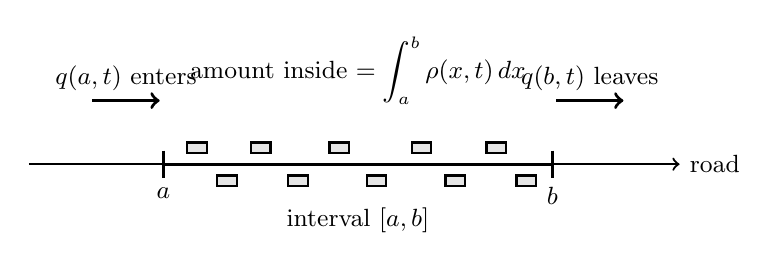
\begin{tikzpicture}[scale=0.95, every node/.style={font=\small}]
  % road
  \draw[->, thick] (-0.5,0) -- (8.2,0) node[right] {road};

  % interval
  \draw[very thick] (1.3,0) -- (6.5,0);
  \draw[thick] (1.3,0.18) -- (1.3,-0.18);
  \draw[thick] (6.5,0.18) -- (6.5,-0.18);

  \node[below] at (1.3,-0.18) {\(a\)};
  \node[below] at (6.5,-0.18) {\(b\)};
  \node[below] at (3.9,-0.45) {interval \([a,b]\)};

  % cars as small rectangles
  \foreach \x/\y in {1.75/0.22,2.15/-0.22,2.6/0.22,3.1/-0.22,3.65/0.22,4.15/-0.22,4.75/0.22,5.2/-0.22,5.75/0.22,6.15/-0.22} {
    \draw[fill=gray!20, thick] (\x-0.13,\y-0.07) rectangle (\x+0.13,\y+0.07);
  }

  % flux arrows
  \draw[very thick,->] (0.35,0.85) -- (1.25,0.85);
  \node[above] at (0.8,0.85) {\(q(a,t)\) enters};

  \draw[very thick,->] (6.55,0.85) -- (7.45,0.85);
  \node[above] at (7.0,0.85) {\(q(b,t)\) leaves};

  \node at (3.9,1.25) {amount inside \(=\displaystyle\int_a^b \rho(x,t)\,dx\)};
\end{tikzpicture}
\caption{In one dimension, an interval has two boundary points.  Flux through those boundary points changes what is inside.}
\label{fig:density-flux-on-line}
\end{figure}

The total number of cars in the road segment \([a,b]\) at time \(t\) is

\[
\boxed{
N(t)=\int_a^b \rho(x,t)\,dx.
}
\]

This is an accumulation of density over length:

\[
\frac{\text{cars}}{\text{mile}}\cdot \text{mile}=\text{cars}.
\]

So the integral turns density into total amount.

\subsection{Accumulation inside an interval}
\label{subsec:accumulation-inside-interval}

Suppose no cars appear or disappear inside the interval \([a,b]\).  There are no
parking lots, no ramps, and no accidents removing cars from the road.  Then the
only way the number of cars inside can change is through the two endpoints.

Cars can enter through the left endpoint \(a\).  The rate of entry is

\[
q(a,t).
\]

Cars can leave through the right endpoint \(b\).  The rate of leaving is

\[
q(b,t).
\]

Therefore

\[
\boxed{
\frac{dN}{dt}=q(a,t)-q(b,t).
}
\]

Since

\[
N(t)=\int_a^b \rho(x,t)\,dx,
\]

we can write this as

\[
\boxed{
\frac{d}{dt}\int_a^b \rho(x,t)\,dx
=
q(a,t)-q(b,t).
}
\]

This is a one-dimensional conservation law.

\begin{quote}
\textbf{Conservation law on an interval.}
If \(\rho(x,t)\) is the density of a conserved quantity and \(q(x,t)\) is the flux to the
right, then, with no sources or sinks inside \([a,b]\),

\[
\boxed{
\frac{d}{dt}\int_a^b \rho(x,t)\,dx
=
q(a,t)-q(b,t).
}
\]

In words:

\[
\boxed{
\text{rate of change inside}=\text{inflow at left}-\text{outflow at right}.
}
\]
\end{quote}

The signs contain the orientation.  Positive flux points to the right.  At the left
endpoint, rightward flux enters the interval.  At the right endpoint, rightward flux
leaves the interval.

\paragraph{Example.}
Suppose cars enter a road segment through \(a\) at

\[
q(a,t)=1200
\]

cars/hour and leave through \(b\) at

\[
q(b,t)=950
\]

cars/hour.  Then

\[
\frac{dN}{dt}=1200-950=250.
\]

So the number of cars in the segment is increasing at

\[
250\text{ cars/hour}.
\]

Traffic is accumulating inside.

\paragraph{Example.}
Suppose instead

\[
q(a,t)=700,
\qquad
q(b,t)=1000.
\]

Then

\[
\frac{dN}{dt}=700-1000=-300.
\]

The number of cars in the segment is decreasing at

\[
300\text{ cars/hour}.
\]

More cars leave than enter.

\paragraph{Sign warning.}
Flux can be negative.  Negative flux means motion to the left.

If

\[
q(a,t)=-100
\]

at the left endpoint, then cars are crossing \(a\) to the left.  They are leaving the
interval through the left endpoint.  The formula still works:

\[
\frac{dN}{dt}=q(a,t)-q(b,t).
\]

The negative value of \(q(a,t)\) correctly decreases \(N(t)\).

\subsection{What crosses the boundary changes what is inside}
\label{subsec:what-crosses-boundary}

The conservation law can be written with the outward boundary in mind.

The interval \([a,b]\) has two outward directions:

\[
\text{left endpoint }a: \text{ outward direction is left},
\]

\[
\text{right endpoint }b: \text{ outward direction is right}.
\]

Since \(q\) is positive to the right, the outward flux is

\[
-q(a,t)
\]

at the left endpoint and

\[
q(b,t)
\]

at the right endpoint.

So the total outward flux is

\[
q(b,t)-q(a,t).
\]

The amount inside decreases when outward flux is positive:

\[
\frac{d}{dt}\int_a^b \rho(x,t)\,dx
=
-\bigl(q(b,t)-q(a,t)\bigr).
\]

This is the same formula as before:

\[
-\bigl(q(b,t)-q(a,t)\bigr)=q(a,t)-q(b,t).
\]

The boundary form is useful because it generalizes.

\[
\boxed{
\text{change inside}=-\text{net outward flow through the boundary}.
}
\]

\paragraph{Sources and sinks.}
The formula above assumes that nothing is created or destroyed inside the interval.
That assumption matters.

Suppose cars can enter through an on-ramp inside \([a,b]\).  Let

\[
s(x,t)=\text{source rate density}
\]

measured in

\[
\text{cars per mile per hour}.
\]

Then the total rate of creation inside the interval is

\[
\int_a^b s(x,t)\,dx.
\]

The conservation law becomes

\[
\boxed{
\frac{d}{dt}\int_a^b \rho(x,t)\,dx
=
q(a,t)-q(b,t)+\int_a^b s(x,t)\,dx.
}
\]

If \(s>0\), cars are being added.  If \(s<0\), cars are being removed.

\begin{quote}
\textbf{Warning.}
Boundary flux alone explains the change inside only when there are no sources or
sinks inside the interval.

If material is created or destroyed inside, the source term must be included.
\end{quote}

This is the same kind of honesty we used throughout calculus.  A theorem's
hypotheses are not decoration.  They say exactly what the formula is allowed to
ignore.

\subsection{Preview of divergence in multivariable calculus}
\label{subsec:preview-divergence-multivariable}

The conservation law on every interval contains a local law.

Start with the no-source case:

\[
\frac{d}{dt}\int_a^b \rho(x,t)\,dx
=
q(a,t)-q(b,t).
\]

If \(\rho\) and \(q\) are smooth enough, we may read the left side as

\[
\int_a^b \frac{\partial \rho}{\partial t}(x,t)\,dx.
\]

The notation

\[
\frac{\partial \rho}{\partial t}
\]

means: differentiate \(\rho(x,t)\) with respect to \(t\), while holding \(x\) fixed.  This
is multivariable notation, but the idea is familiar.

The right side can be rewritten using the Fundamental Theorem:

\[
q(a,t)-q(b,t)
=
-\bigl(q(b,t)-q(a,t)\bigr)
=
-\int_a^b \frac{\partial q}{\partial x}(x,t)\,dx.
\]

Therefore

\[
\int_a^b \frac{\partial \rho}{\partial t}(x,t)\,dx
=
-\int_a^b \frac{\partial q}{\partial x}(x,t)\,dx.
\]

Bring everything to one side:

\[
\int_a^b
\left(
\frac{\partial \rho}{\partial t}
+
\frac{\partial q}{\partial x}
\right)
dx=0.
\]

If this holds for every interval \([a,b]\), then the integrand must be zero:

\[
\boxed{
\frac{\partial \rho}{\partial t}
+
\frac{\partial q}{\partial x}
=
0.
}
\]

This is the local form of conservation in one dimension.

\begin{quote}
\textbf{One-dimensional conservation law, local form.}
With no sources or sinks,

\[
\boxed{
\rho_t+q_x=0.
}
\]

With source term \(s\),

\[
\boxed{
\rho_t+q_x=s.
}
\]
\end{quote}

Here

\[
\rho_t=\frac{\partial \rho}{\partial t},
\qquad
q_x=\frac{\partial q}{\partial x}.
\]

What does \(q_x\) mean physically?

Look at a tiny interval from \(x\) to \(x+\Delta x\).  The flux entering from the left is
approximately

\[
q(x,t),
\]

and the flux leaving to the right is approximately

\[
q(x+\Delta x,t).
\]

The net outward flux is

\[
q(x+\Delta x,t)-q(x,t).
\]

Divide by the length \(\Delta x\):

\[
\frac{q(x+\Delta x,t)-q(x,t)}{\Delta x}.
\]

As \(\Delta x\to0\), this approaches

\[
q_x(x,t).
\]

So \(q_x\) measures local net outward flow per unit length.

If

\[
q_x>0,
\]

more is leaving a tiny interval than entering it, so density tends to decrease.  If

\[
q_x<0,
\]

more is entering than leaving, so density tends to increase.

\begin{figure}[h]
\centering
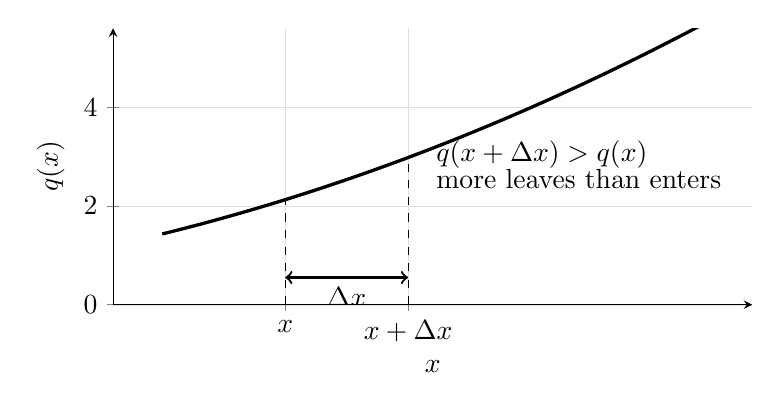
\begin{tikzpicture}
\begin{axis}[
    width=0.80\textwidth,
    height=0.42\textwidth,
    xmin=0, xmax=5.2,
    ymin=0, ymax=5.6,
    axis lines=left,
    xlabel={\(x\)},
    ylabel={\(q(x)\)},
    xtick={1.4,2.4},
    xticklabels={\(x\),\(x+\Delta x\)},
    ytick={0,2,4},
    grid=both,
    grid style={line width=.1pt, draw=gray!25},
]
\addplot[very thick, domain=0.4:4.8, samples=100] {1.2+0.55*x+0.08*x^2};
\draw[dashed] (axis cs:1.4,0) -- (axis cs:1.4,2.1268);
\draw[dashed] (axis cs:2.4,0) -- (axis cs:2.4,2.9808);
\draw[<->, thick] (axis cs:1.4,0.55) -- (axis cs:2.4,0.55);
\node[anchor=north] at (axis cs:1.9,0.55) {\(\Delta x\)};
\node[anchor=west] at (axis cs:2.55,3.05) {\(q(x+\Delta x)>q(x)\)};
\node[anchor=west] at (axis cs:2.55,2.55) {more leaves than enters};
\end{axis}
\end{tikzpicture}
\caption{When \(q\) increases with \(x\), the outgoing flux from a small interval exceeds the incoming flux.}
\label{fig:flux-derivative-divergence-1d}
\end{figure}

In multivariable calculus, the flux becomes a vector field.  Instead of moving only left
or right, material can flow in many directions.  The derivative \(q_x\) becomes
\emph{divergence}:

\[
\nabla\cdot \mathbf{q}.
\]

The conservation law becomes

\[
\boxed{
\rho_t+\nabla\cdot\mathbf{q}=s.
}
\]

The idea is the same as the one-dimensional version:

\[
\boxed{
\text{local change in density}
+
\text{local net outward flow}
=
\text{local creation}.
}
\]

This is why the boundary viewpoint matters.  The Fundamental Theorem, flux through
endpoints, conservation laws, and divergence are not separate tricks.  They are stages
of one story:

\[
\text{inside} \quad \longleftrightarrow \quad \text{boundary}.
\]

There is one final bridge.  Calculus has optimized numbers: shortest distance, largest
area, greatest profit.  But physics and geometry often ask for the best \emph{path}.  That
means optimizing a whole function.

\section{Least action and the shape of a path}
\label{sec:least-action-shape-path}

Optimization began with numbers.  We chose a radius, a price, a time, or a point and
made a function as large or as small as possible.

But a path is not one number.  A path is a whole function.

A bead sliding along a wire chooses a curve.  Light traveling through different media
chooses a path.  A planet moving under gravity traces an orbit.  The question is no
longer

\[
\text{Which number is best?}
\]

but

\[
\boxed{
\text{Which function is best?}
}
\]

That question leads beyond ordinary single-variable calculus.  Still, the first idea is
visible with tools we already know: derivatives, integrals, and integration by parts.

\subsection{From optimization of numbers to optimization of functions}
\label{subsec:optimization-numbers-to-functions}

A usual optimization problem starts with a function such as

\[
A(r)=\pi r^2
\]

or

\[
P(x)=\text{profit at price }x.
\]

The input is a number.  We find a best number by solving

\[
A'(r)=0
\qquad\text{or}\qquad
P'(x)=0,
\]

then checking the result.

A path problem is different.  The input is a function.

For example, a curve from \((a,A)\) to \((b,B)\) might be written as

\[
y=y(x),
\qquad
a\le x\le b,
\]

with endpoint conditions

\[
y(a)=A,
\qquad
y(b)=B.
\]

The length of that curve is

\[
\mathcal{L}[y]
=
\int_a^b \sqrt{1+\bigl(y'(x)\bigr)^2}\,dx.
\]

The square brackets remind us that \(\mathcal{L}\) eats a whole function \(y\), not just
one number.  Such an object is called a \emph{functional}.

\begin{quote}
\textbf{Functional.}
A \emph{functional} is a rule that assigns a number to a function.

For example,

\[
\mathcal{L}[y]
=
\int_a^b \sqrt{1+\bigl(y'(x)\bigr)^2}\,dx
\]

assigns to a path \(y(x)\) its arc length.
\end{quote}

To test whether a function is best, we wiggle it slightly.

Let \(\eta(x)\) be a small ``wiggle'' function satisfying

\[
\eta(a)=0,
\qquad
\eta(b)=0.
\]

These conditions keep the endpoints fixed.  For a small number \(\varepsilon\), form the
nearby path

\[
y_\varepsilon(x)=y(x)+\varepsilon\eta(x).
\]

If \(y\) is the best path, then changing \(\varepsilon\) away from \(0\) should not improve
the value, at least to first order.  So we expect

\[
\left.\frac{d}{d\varepsilon}\mathcal{L}[y+\varepsilon\eta]\right|_{\varepsilon=0}=0
\]

for every allowed wiggle \(\eta\).

\begin{figure}[h]
\centering
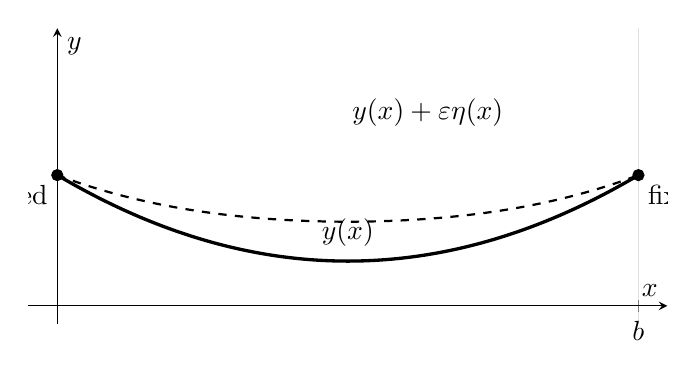
\begin{tikzpicture}
\begin{axis}[
    width=0.80\textwidth,
    height=0.44\textwidth,
    xmin=-0.2, xmax=4.2,
    ymin=-0.1, ymax=1.55,
    axis lines=middle,
    xlabel={\(x\)},
    ylabel={\(y\)},
    xtick={0,4},
    xticklabels={\(a\),\(b\)},
    ytick=\empty,
    grid=both,
    grid style={line width=.1pt, draw=gray!25},
]
\addplot[very thick, domain=0:4, samples=200] {0.12*(x-2)^2+0.25};
\addplot[thick, dashed, domain=0:4, samples=200] {0.12*(x-2)^2+0.25+0.22*sin(45*x)};
\addplot[only marks, mark=*] coordinates {(0,0.73) (4,0.73)};
\node[anchor=south] at (axis cs:2.0,0.28) {\(y(x)\)};
\node[anchor=south] at (axis cs:2.55,0.95) {\(y(x)+\varepsilon\eta(x)\)};
\node[anchor=north east] at (axis cs:0,0.73) {fixed};
\node[anchor=north west] at (axis cs:4,0.73) {fixed};
\end{axis}
\end{tikzpicture}
\caption{To optimize a path, we compare it with nearby paths that keep the endpoints fixed.}
\label{fig:path-variation}
\end{figure}

This is the function-level analogue of the condition

\[
f'(c)=0
\]

from ordinary optimization.

The derivative is now taken with respect to the wiggle size \(\varepsilon\).  The unknown
object is the whole path \(y\).

\subsection{The brachistochrone story}
\label{subsec:brachistochrone-story}

One of the most famous path problems asks for the fastest slide.

Place a bead at a point \(A\).  Let it slide without friction under gravity to a lower
point \(B\).  We may choose the shape of the wire connecting \(A\) to \(B\).

Which wire gives the shortest travel time?

The shortest path is a straight line.  But the fastest path is not a straight line.  A path
that drops steeply at first lets the bead gain speed quickly, and that speed can help
later.

This is the \emph{brachistochrone problem}.  The word comes from Greek roots meaning
``shortest time.''

Let \(y\) measure vertical distance downward from the starting height.  Then \(y>0\)
means the bead has fallen.  If the bead starts from rest, conservation of energy gives

\[
\frac12mv^2=mgy.
\]

So the speed is

\[
v=\sqrt{2gy}.
\]

A small piece of arc length is

\[
ds=\sqrt{1+(y')^2}\,dx.
\]

Since

\[
\text{time}=\frac{\text{distance}}{\text{speed}},
\]

the small time is

\[
dT=\frac{ds}{v}
=
\frac{\sqrt{1+(y')^2}}{\sqrt{2gy}}\,dx.
\]

Thus the total travel time is the functional

\[
\boxed{
T[y]
=
\int_a^b
\frac{\sqrt{1+(y')^2}}{\sqrt{2gy}}\,dx.
}
\]

The problem is to find the function \(y(x)\) that makes this integral as small as possible,
with fixed endpoints.

That is not an ordinary optimization problem.  The input is the whole curve.

The answer is beautiful: the fastest curve is an arc of a \emph{cycloid}, the curve traced
by a point on the rim of a rolling circle.

One convenient cycloid parametrization is

\[
x=r(\theta-\sin\theta),
\qquad
y=r(1-\cos\theta),
\]

where \(y\) is measured downward.

\begin{figure}[h]
\centering
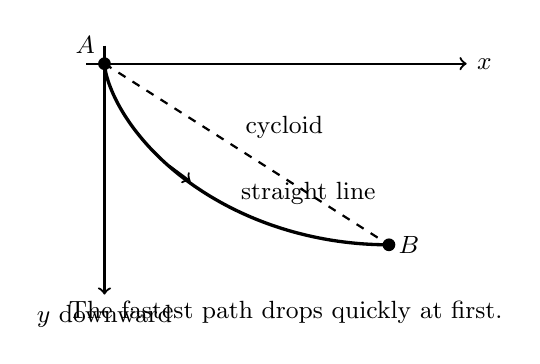
\begin{tikzpicture}[scale=1.15, every node/.style={font=\small}]
  \def\PI{3.14159}

  % axes: y downward
  \draw[->, thick] (-0.2,0) -- (4.0,0) node[right] {\(x\)};
  \draw[->, thick] (0,0.2) -- (0,-2.55) node[below] {\(y\) downward};

  % straight line
  \draw[thick, dashed] (0,0) -- (\PI,-2);

  % cycloid r=1, theta 0 to 180
  \draw[very thick, domain=0:180, samples=200, smooth, variable=\t]
    plot ({(\t/180)*\PI - sin(\t)}, {-(1-cos(\t))});

  % endpoints
  \fill (0,0) circle (2pt);
  \fill (\PI,-2) circle (2pt);

  \node[above left] at (0,0) {\(A\)};
  \node[right] at (\PI,-2) {\(B\)};

  \node[above right] at (1.45,-0.93) {cycloid};
  \node[below right] at (1.4,-1.2) {straight line};

  % direction arrow on cycloid
  \draw[->, thick] (0.72,-1.13) -- (0.95,-1.30);

  \node at (2.0,-2.75) {The fastest path drops quickly at first.};
\end{tikzpicture}
\caption{The brachistochrone is not the shortest path.  It is the path of shortest time.}
\label{fig:brachistochrone-cycloid}
\end{figure}

For the special cycloid

\[
x=\theta-\sin\theta,
\qquad
y=1-\cos\theta,
\qquad
0\le \theta\le \pi,
\]

the endpoint is

\[
B=(\pi,2).
\]

Along this cycloid,

\[
\frac{ds}{d\theta}=2\sin\frac{\theta}{2},
\]

and

\[
\sqrt{2gy}
=
\sqrt{2g(1-\cos\theta)}
=
2\sqrt{g}\sin\frac{\theta}{2}.
\]

Therefore

\[
dT=\frac{ds}{v}
=
\frac{2\sin(\theta/2)\,d\theta}
{2\sqrt{g}\sin(\theta/2)}
=
\frac{1}{\sqrt g}\,d\theta.
\]

So the cycloid travel time from \(\theta=0\) to \(\theta=\pi\) is

\[
\boxed{
T_{\text{cycloid}}=\frac{\pi}{\sqrt g}.
}
\]

The straight line from \((0,0)\) to \((\pi,2)\) has equation

\[
y=\frac{2}{\pi}x.
\]

Its travel time works out to

\[
\boxed{
T_{\text{line}}
=
\frac{\pi}{\sqrt g}\sqrt{1+\frac{4}{\pi^2}}.
}
\]

Since

\[
\sqrt{1+\frac{4}{\pi^2}}>1,
\]

we have

\[
T_{\text{line}}>T_{\text{cycloid}}.
\]

The straight line is shorter, but slower.

\begin{quote}
\textbf{Lesson of the brachistochrone.}
The best path depends on what is being optimized.

Shortest distance and shortest time are different questions.
\end{quote}

The full proof that the cycloid is the fastest curve belongs to the calculus of variations.
But the setup already shows the new kind of calculus: an integral depends on a path, and
we seek the path that makes the integral extreme.

\subsection{A gentle first variation calculation}
\label{subsec:gentle-first-variation-calculation}

The brachistochrone is famous but technically demanding.  The easiest variational
problem is the shortest path between two points.

We know the answer geometrically: the shortest path is a straight line.  Let us see how
calculus finds that answer.

Let \(y(x)\) be a path from \((a,A)\) to \((b,B)\).  Its length is

\[
\mathcal{L}[y]
=
\int_a^b \sqrt{1+\bigl(y'(x)\bigr)^2}\,dx.
\]

Let \(\eta(x)\) be any smooth wiggle with

\[
\eta(a)=0,
\qquad
\eta(b)=0.
\]

Consider nearby paths

\[
y_\varepsilon(x)=y(x)+\varepsilon\eta(x).
\]

Their lengths are

\[
\mathcal{L}(\varepsilon)
=
\int_a^b
\sqrt{1+\bigl(y'(x)+\varepsilon\eta'(x)\bigr)^2}
\,dx.
\]

If \(y\) is a shortest path, then \(\varepsilon=0\) should be a minimum of
\(\mathcal{L}(\varepsilon)\).  Therefore

\[
\mathcal{L}'(0)=0.
\]

Differentiate with respect to \(\varepsilon\):

\[
\mathcal{L}'(\varepsilon)
=
\int_a^b
\frac{\bigl(y'+\varepsilon\eta'\bigr)\eta'}
{\sqrt{1+\bigl(y'+\varepsilon\eta'\bigr)^2}}
\,dx.
\]

Set \(\varepsilon=0\):

\[
\mathcal{L}'(0)
=
\int_a^b
\frac{y'\eta'}{\sqrt{1+(y')^2}}
\,dx.
\]

For a shortest path, this must be zero for every allowed wiggle \(\eta\):

\[
\int_a^b
\frac{y'\eta'}{\sqrt{1+(y')^2}}
\,dx=0.
\]

Now use integration by parts.  Let

\[
u=\frac{y'}{\sqrt{1+(y')^2}},
\qquad
dv=\eta'\,dx.
\]

Then

\[
v=\eta.
\]

So

\[
\int_a^b
\frac{y'\eta'}{\sqrt{1+(y')^2}}
\,dx
=
\left[
\frac{y'}{\sqrt{1+(y')^2}}\eta
\right]_a^b
-
\int_a^b
\frac{d}{dx}
\left(
\frac{y'}{\sqrt{1+(y')^2}}
\right)
\eta\,dx.
\]

The boundary term vanishes because

\[
\eta(a)=\eta(b)=0.
\]

Therefore

\[
\mathcal{L}'(0)
=
-
\int_a^b
\frac{d}{dx}
\left(
\frac{y'}{\sqrt{1+(y')^2}}
\right)
\eta\,dx.
\]

For this to be zero for every allowed wiggle \(\eta\), the coefficient of \(\eta\) must be
zero:

\[
\frac{d}{dx}
\left(
\frac{y'}{\sqrt{1+(y')^2}}
\right)
=0.
\]

Thus

\[
\frac{y'}{\sqrt{1+(y')^2}}
\]

is constant.  This forces \(y'\) itself to be constant.  Therefore

\[
y'=m
\]

for some constant \(m\), and hence

\[
\boxed{
y=mx+c.
}
\]

The shortest path is a straight line.

\begin{quote}
\textbf{What the calculation did.}
We did not vary a number.  We varied a whole path:

\[
y\quad\longrightarrow\quad y+\varepsilon\eta.
\]

Then we required the first-order change to vanish for every endpoint-fixed wiggle
\(\eta\).
\end{quote}

The boundary condition on \(\eta\) matters.  If the endpoints were not fixed, the
boundary term from integration by parts would not disappear.  Once again, boundary
terms carry real information.

\subsection{Why this is beyond ordinary single-variable calculus}
\label{subsec:why-variation-beyond-single-variable}

A functional often has the form

\[
\mathcal{J}[y]
=
\int_a^b L(x,y,y')\,dx.
\]

The function \(L\) is called a \emph{Lagrangian}.  It tells how the path and its slope
contribute to the accumulated quantity.

The first variation calculation leads to the Euler--Lagrange equation:

\[
\boxed{
\frac{\partial L}{\partial y}
-
\frac{d}{dx}
\left(
\frac{\partial L}{\partial y'}
\right)
=0.
}
\]

This formula belongs to the calculus of variations.  It is a cousin of the ordinary
condition

\[
f'(c)=0,
\]

but it applies when the unknown is a function.

For the shortest path problem,

\[
L(x,y,y')=\sqrt{1+(y')^2}.
\]

Since \(L\) does not depend directly on \(y\),

\[
\frac{\partial L}{\partial y}=0.
\]

The Euler--Lagrange equation becomes

\[
\frac{d}{dx}
\left(
\frac{y'}{\sqrt{1+(y')^2}}
\right)
=0,
\]

the equation we found by hand.

\paragraph{Least action.}
Physics uses the same idea in time.

Suppose a particle moves along a line, with position \(x(t)\).  Its kinetic energy is

\[
\frac12m(x')^2,
\]

and its potential energy is

\[
V(x).
\]

Define the action

\[
\boxed{
\mathcal{S}[x]
=
\int_{t_0}^{t_1}
\left(
\frac12m(x')^2-V(x)
\right)
dt.
}
\]

The principle of least action says, historically, that the physical path makes this
quantity ``least.''  The more accurate statement is that the physical path makes the
first variation of the action equal to zero.  It makes the action \emph{stationary}.

Let

\[
x_\varepsilon(t)=x(t)+\varepsilon\eta(t),
\]

where the wiggle fixes the endpoints:

\[
\eta(t_0)=\eta(t_1)=0.
\]

Differentiate the action with respect to \(\varepsilon\) at \(\varepsilon=0\):

\[
\left.\frac{d}{d\varepsilon}\mathcal{S}[x+\varepsilon\eta]\right|_{\varepsilon=0}
=
\int_{t_0}^{t_1}
\left(
m x'\eta' - V'(x)\eta
\right)
dt.
\]

Use integration by parts on the first term:

\[
\int_{t_0}^{t_1}m x'\eta'\,dt
=
\left[mx'\eta\right]_{t_0}^{t_1}
-
\int_{t_0}^{t_1}m x''\eta\,dt.
\]

The boundary term vanishes because the endpoints are fixed.  Therefore

\[
\left.\frac{d}{d\varepsilon}\mathcal{S}[x+\varepsilon\eta]\right|_{\varepsilon=0}
=
-
\int_{t_0}^{t_1}
\bigl(mx''+V'(x)\bigr)\eta\,dt.
\]

For this to be zero for every allowed wiggle \(\eta\), we need

\[
mx''+V'(x)=0.
\]

So

\[
\boxed{
mx''=-V'(x).
}
\]

That is Newton's second law for a force

\[
F(x)=-V'(x).
\]

A law of motion has emerged from an optimization principle.

\begin{quote}
\textbf{Stationary does not always mean minimum.}
The historical phrase is ``least action,'' but the safest calculus statement is

\[
\text{the first variation is zero.}
\]

This is like ordinary calculus: \(f'(c)=0\) may indicate a minimum, a maximum, or
neither.  More work is needed to decide which.
\end{quote}

This is why the subject goes beyond the ordinary single-variable course.  We need to
make sense of spaces of functions, allowed variations, endpoint conditions, existence of
minimizers, and the difference between minimum and stationary.

But the seed is already here:

\[
\boxed{
\text{differentiate an accumulated quantity, watch the boundary terms, and set the first variation to zero.}
}
\]

That sentence connects much of the road ahead.  In multivariable calculus, the
boundary of an interval becomes the boundary of a region.  Flux through endpoints
becomes flux through curves and surfaces.  The Fundamental Theorem becomes
Green's theorem, the Divergence Theorem, and Stokes' theorem.

The book began with distance and velocity.  It ends by pointing to the same pattern in
larger geometry:

\[
\boxed{
\text{change inside is measured by derivatives and boundaries.}
}
\]

\section{Final projects}
\label{sec:final-projects}

The book began with two instruments on a dashboard.  One measured accumulated
distance.  The other measured instantaneous change.

Since then, the same two ideas have appeared in many forms:

\[
\text{derivatives measure local change},
\qquad
\text{integrals accumulate small pieces}.
\]

Taylor polynomials turned local derivative information into approximations.  Differential
equations turned laws of change into unknown functions.  Parametric curves let motion
draw geometry.  Fourier ideas built periodic motion from waves.  The one-dimensional
Stokes theorem revealed the Fundamental Theorem as a boundary theorem.

These final projects ask you to use the whole story.

\begin{figure}[h]
\centering
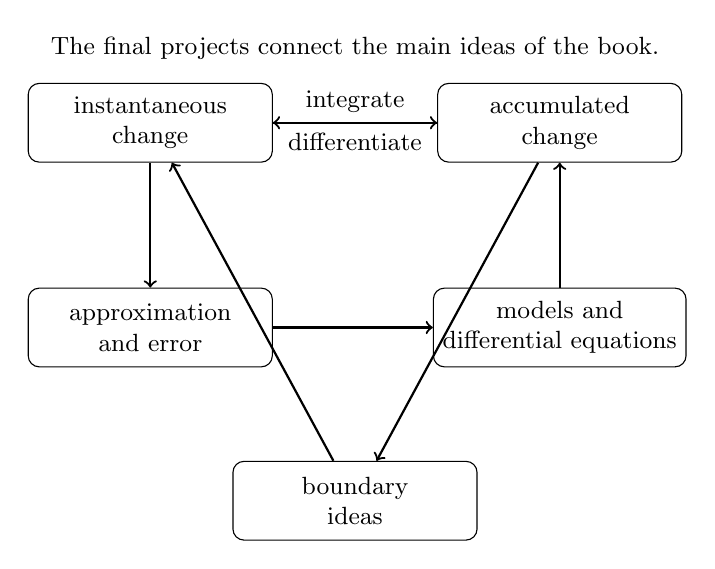
\begin{tikzpicture}[every node/.style={font=\small}, scale=1]
  \node[draw, rounded corners, align=center, minimum width=3.1cm, minimum height=1cm] (change) at (0,2.3)
  {instantaneous\\change};

  \node[draw, rounded corners, align=center, minimum width=3.1cm, minimum height=1cm] (accum) at (5.2,2.3)
  {accumulated\\change};

  \node[draw, rounded corners, align=center, minimum width=3.1cm, minimum height=1cm] (approx) at (0,-0.3)
  {approximation\\and error};

  \node[draw, rounded corners, align=center, minimum width=3.1cm, minimum height=1cm] (models) at (5.2,-0.3)
  {models and\\differential equations};

  \node[draw, rounded corners, align=center, minimum width=3.1cm, minimum height=1cm] (boundary) at (2.6,-2.5)
  {boundary\\ideas};

  \draw[->, thick] (change) -- node[above] {integrate} (accum);
  \draw[->, thick] (accum) -- node[below] {differentiate} (change);

  \draw[->, thick] (change) -- (approx);
  \draw[->, thick] (approx) -- (models);
  \draw[->, thick] (models) -- (accum);

  \draw[->, thick] (accum) -- (boundary);
  \draw[->, thick] (boundary) -- (change);

  \node[align=center] at (2.6,3.25)
  {The final projects connect the main ideas of the book.};
\end{tikzpicture}
\caption{Calculus is one connected language: change, accumulation, approximation, models, and boundary terms.}
\label{fig:final-project-map}
\end{figure}

Each project below can be done alone or with a small group.  A good solution should
include clear calculations, graphs when they help, and a short written explanation of what
the calculations mean.

\subsection{Model, solve, and test a cooling law}
\label{subsec:project-cooling-law}

Newton's law of cooling was one of our first differential equation models:

\[
T'=-k(T-T_s).
\]

It says that the rate of cooling is proportional to the temperature difference between the
object and its surroundings.

This project asks you to build the model from data, solve it, and then test whether it
deserves to be trusted.

\begin{quote}
\textbf{Project question.}
A cup of coffee is placed in a room whose temperature is

\[
T_s=22^\circ\text{C}.
\]

The coffee temperature is recorded every \(5\) minutes.

\begin{center}
\renewcommand{\arraystretch}{1.25}
\begin{tabular}{c|ccccccc}
\(t\) (minutes) & \(0\) & \(5\) & \(10\) & \(15\) & \(20\) & \(25\) & \(30\) \\ \hline
\(T(t)\) \((^\circ\text{C})\) & \(86\) & \(71\) & \(59\) & \(50\) & \(43\) & \(38\) & \(34\)
\end{tabular}
\end{center}

Does Newton's law of cooling give a reasonable model for this data?
\end{quote}

\paragraph{Part A: solve the model.}
Start from

\[
T'=-k(T-T_s).
\]

Let

\[
u=T-T_s.
\]

Then

\[
u'=T',
\]

so the differential equation becomes

\[
u'=-ku.
\]

Therefore

\[
u(t)=Ce^{-kt}.
\]

Since

\[
u(t)=T(t)-T_s,
\]

the temperature model is

\[
\boxed{
T(t)=T_s+Ce^{-kt}.
}
\]

Using the initial temperature \(T(0)=86\), find \(C\).

\paragraph{Part B: estimate the cooling constant.}
Use the first and last data points to estimate \(k\).  Since

\[
T(t)-T_s=Ce^{-kt},
\]

we have

\[
\frac{T(t_2)-T_s}{T(t_1)-T_s}
=
e^{-k(t_2-t_1)}.
\]

Taking logarithms gives

\[
\boxed{
k
=
-\frac{1}{t_2-t_1}
\ln
\left(
\frac{T(t_2)-T_s}{T(t_1)-T_s}
\right).
}
\]

Using \(t_1=0\) and \(t_2=30\),

\[
k
\approx
-\frac1{30}
\ln
\left(
\frac{34-22}{86-22}
\right).
\]

Compute this value.  Then write the complete model

\[
T(t)=22+Ce^{-kt}.
\]

\paragraph{Part C: linearize the data.}
The model predicts

\[
T(t)-T_s=Ce^{-kt}.
\]

Taking logarithms gives

\[
\boxed{
\ln(T(t)-T_s)=\ln C-kt.
}
\]

So if Newton's law is a good model, the points

\[
\bigl(t,\ln(T(t)-22)\bigr)
\]

should lie approximately on a line.

Make a table of

\[
\ln(T(t)-22)
\]

for the data.  Plot these transformed points.  Estimate the slope of the line and compare
it with \(-k\).

\paragraph{Part D: test the model.}
For each recorded time \(t_j\), compute the model prediction

\[
T_{\text{model}}(t_j)=22+Ce^{-kt_j}.
\]

Then compute the residual

\[
R_j=T_{\text{data}}(t_j)-T_{\text{model}}(t_j).
\]

Record your results in a table.

\begin{center}
\renewcommand{\arraystretch}{1.35}
\begin{tabular}{c|c|c|c}
\textbf{time} \(t_j\) &
\textbf{data} \(T_{\text{data}}(t_j)\) &
\textbf{model} \(T_{\text{model}}(t_j)\) &
\textbf{residual} \(R_j\) \\ \hline
 & & & \\
 & & & \\
 & & &
\end{tabular}
\end{center}

Plot the residuals.  A good model should not show a strong pattern in the residuals.
If the residuals are all positive early and all negative later, the model is missing
something systematic.

\paragraph{Part E: interpret the result.}
Write a short conclusion answering these questions.

\begin{enumerate}
\item What value of \(k\) did you find, and what are its units?

\item According to your model, when will the coffee reach \(40^\circ\text{C}\)?

\item Does the transformed logarithm plot look approximately linear?

\item Are the residuals small compared with the temperature changes?

\item What physical effects might make the model imperfect?
\end{enumerate}

A model is not good because it has a formula.  A model is good when it explains the
data well enough for the question being asked.

\subsection{Approximate a difficult integral three ways}
\label{subsec:project-approximate-difficult-integral}

Some integrals exist clearly but do not have elementary antiderivatives.  The integral

\[
I=\int_0^1 e^{-x^2}\,dx
\]

is one of the most important examples.

The function

\[
e^{-x^2}
\]

is continuous and positive on \([0,1]\), so the integral exists.  But no elementary
function has derivative \(e^{-x^2}\).  The Fundamental Theorem still tells us what an
antiderivative would do, but it does not supply one from our usual list.

So we approximate.

\begin{quote}
\textbf{Project question.}
Approximate

\[
\boxed{
I=\int_0^1 e^{-x^2}\,dx
}
\]

using three numerical methods, compare the answers, and give an error discussion.
\end{quote}

\paragraph{Part A: midpoint rule.}
Divide \([0,1]\) into \(n\) equal subintervals of width

\[
\Delta x=\frac1n.
\]

The midpoint rule is

\[
\boxed{
M_n
=
\Delta x
\sum_{j=1}^{n}
f\left(\frac{x_{j-1}+x_j}{2}\right),
}
\]

where

\[
f(x)=e^{-x^2}.
\]

Compute \(M_n\) for

\[
n=4,\quad 8,\quad 16,\quad 32.
\]

\paragraph{Part B: trapezoidal rule.}
The trapezoidal rule is

\[
\boxed{
T_n
=
\frac{\Delta x}{2}
\left[
f(x_0)+2f(x_1)+2f(x_2)+\cdots+2f(x_{n-1})+f(x_n)
\right].
}
\]

Compute \(T_n\) for

\[
n=4,\quad 8,\quad 16,\quad 32.
\]

\paragraph{Part C: Simpson's rule.}
For even \(n\), Simpson's rule is

\[
\boxed{
S_n
=
\frac{\Delta x}{3}
\left[
f(x_0)
+
4f(x_1)
+
2f(x_2)
+
4f(x_3)
+\cdots+
2f(x_{n-2})
+
4f(x_{n-1})
+
f(x_n)
\right].
}
\]

Compute \(S_n\) for

\[
n=4,\quad 8,\quad 16,\quad 32.
\]

\paragraph{Part D: organize the results.}
Make a table.

\begin{center}
\renewcommand{\arraystretch}{1.35}
\begin{tabular}{c|c|c|c}
\(\boldsymbol{n}\) & \(\boldsymbol{M_n}\) & \(\boldsymbol{T_n}\) & \(\boldsymbol{S_n}\) \\ \hline
\(4\) & & & \\
\(8\) & & & \\
\(16\) & & & \\
\(32\) & & &
\end{tabular}
\end{center}

Which column appears to settle fastest?

\paragraph{Part E: use error bounds.}
For

\[
f(x)=e^{-x^2}
\]

on \([0,1]\), you may use the bounds

\[
|f''(x)|\le 2
\]

and

\[
|f^{(4)}(x)|\le 12.
\]

The midpoint and trapezoidal error estimates are

\[
\boxed{
|E_M|
\le
\frac{K(b-a)^3}{24n^2}
}
\]

and

\[
\boxed{
|E_T|
\le
\frac{K(b-a)^3}{12n^2},
}
\]

where

\[
|f''(x)|\le K.
\]

Simpson's rule has the error estimate

\[
\boxed{
|E_S|
\le
\frac{K(b-a)^5}{180n^4},
}
\]

where

\[
|f^{(4)}(x)|\le K.
\]

Use these formulas to give guaranteed error bounds for \(M_{32}\), \(T_{32}\), and
\(S_{32}\).

\paragraph{Optional extension: Taylor series method.}
Use the Taylor series

\[
e^{-x^2}
=
1-x^2+\frac{x^4}{2!}-\frac{x^6}{3!}
+\frac{x^8}{4!}-\cdots.
\]

Integrate term by term on \([0,1]\):

\[
\int_0^1 e^{-x^2}\,dx
=
1-\frac13+\frac{1}{2!\,5}
-\frac{1}{3!\,7}
+\frac{1}{4!\,9}
-\cdots.
\]

Compare this series approximation with your numerical approximations.

\paragraph{Final report.}
Your report should include:

\begin{enumerate}
\item the three approximation tables;
\item at least one graph of \(y=e^{-x^2}\) on \([0,1]\);
\item a comparison of midpoint, trapezoidal, and Simpson approximations;
\item a clear error statement for your best approximation;
\item a paragraph explaining why numerical integration is needed here.
\end{enumerate}

A decimal answer without an error statement is unfinished calculus.

\subsection{Build a Taylor-series calculator}
\label{subsec:project-taylor-series-calculator}

A calculator evaluates functions so quickly that it is easy to forget the question:

\[
\text{How does the calculator know the value?}
\]

For many functions, one answer is Taylor series.  The calculator does not store every
value of \(\sin x\), \(e^x\), or \(\cos x\).  It uses algorithms, and Taylor polynomials are
one of the first algorithms we can understand.

\begin{quote}
\textbf{Project question.}
Build a Taylor-series calculator for one or more elementary functions, and test its
accuracy.
\end{quote}

Choose at least one of the following functions.

\begin{center}
\renewcommand{\arraystretch}{1.45}
\begin{tabular}{c|c|c}
\textbf{function} & \textbf{series centered at \(0\)} & \textbf{natural domain for project} \\ \hline
\(e^x\) &
\(\displaystyle \sum_{n=0}^{\infty}\frac{x^n}{n!}\) &
\(-3\le x\le3\) \\

\(\sin x\) &
\(\displaystyle \sum_{n=0}^{\infty}(-1)^n\frac{x^{2n+1}}{(2n+1)!}\) &
\(-\pi\le x\le\pi\) \\

\(\cos x\) &
\(\displaystyle \sum_{n=0}^{\infty}(-1)^n\frac{x^{2n}}{(2n)!}\) &
\(-\pi\le x\le\pi\) \\

\(\ln(1+x)\) &
\(\displaystyle \sum_{n=1}^{\infty}(-1)^{n+1}\frac{x^n}{n}\) &
\(-1<x\le1\) \\

\(\arctan x\) &
\(\displaystyle \sum_{n=0}^{\infty}(-1)^n\frac{x^{2n+1}}{2n+1}\) &
\(-1\le x\le1\)
\end{tabular}
\end{center}

\paragraph{Part A: write the partial sums.}
For your chosen function, define the \(N\)-th Taylor approximation.

For example, for \(\sin x\),

\[
S_N(x)
=
\sum_{n=0}^{N}
(-1)^n\frac{x^{2n+1}}{(2n+1)!}.
\]

For \(\cos x\),

\[
C_N(x)
=
\sum_{n=0}^{N}
(-1)^n\frac{x^{2n}}{(2n)!}.
\]

\paragraph{Part B: avoid recomputing factorials.}
A practical calculator should not recompute every factorial from scratch.  Use a recurrence
for the terms.

For \(e^x\), if

\[
a_n=\frac{x^n}{n!},
\]

then

\[
\boxed{
a_{n+1}=a_n\frac{x}{n+1}.
}
\]

For \(\sin x\), if

\[
a_n=(-1)^n\frac{x^{2n+1}}{(2n+1)!},
\]

then

\[
\boxed{
a_{n+1}
=
-a_n
\frac{x^2}{(2n+2)(2n+3)}.
}
\]

For \(\cos x\), if

\[
a_n=(-1)^n\frac{x^{2n}}{(2n)!},
\]

then

\[
\boxed{
a_{n+1}
=
-a_n
\frac{x^2}{(2n+1)(2n+2)}.
}
\]

Use a similar recurrence for your chosen series.

\paragraph{Part C: choose a stopping rule.}
Pick a tolerance such as

\[
10^{-4},\qquad 10^{-6},\qquad \text{or}\qquad 10^{-8}.
\]

For alternating series with decreasing term sizes, the alternating series estimate gives

\[
\boxed{
|\text{error}|\le \text{first omitted term}.
}
\]

That applies cleanly to many values of \(\sin x\), \(\cos x\), \(\ln(1+x)\), and
\(\arctan x\), but only when the term sizes are decreasing.

For \(e^x\), use the Lagrange remainder estimate:

\[
\boxed{
|R_N(x)|
\le
\frac{e^B |x|^{N+1}}{(N+1)!}
}
\]

when

\[
|x|\le B.
\]

On the interval \([-3,3]\), you may use \(B=3\).

\paragraph{Part D: test the calculator.}
Choose at least \(8\) input values in the interval.  For each one, record:

\begin{enumerate}
\item the Taylor approximation;
\item the number of terms used;
\item the value from a calculator or computer;
\item the absolute error.
\end{enumerate}

Use a table.

\begin{center}
\renewcommand{\arraystretch}{1.35}
\begin{tabular}{c|c|c|c|c}
\(\boldsymbol{x}\) &
\textbf{Taylor approximation} &
\textbf{terms used} &
\textbf{reference value} &
\textbf{absolute error} \\ \hline
 & & & & \\
 & & & & \\
 & & & &
\end{tabular}
\end{center}

\paragraph{Part E: graph the error.}
Let \(P_N(x)\) be your Taylor approximation.  Plot

\[
E_N(x)=|f(x)-P_N(x)|
\]

on the interval.  Make several plots using different values of \(N\).

Explain where the approximation is best and where it is worst.

\paragraph{Warning: small terms are not always enough.}
A common mistake is to stop when the next term is small, without knowing whether the
tail is controlled.  For alternating series with decreasing terms, that is justified.  For
other series, it may not be.

A calculator must be fast, but it must also be honest.

\subsection{Analyze a parametric curve from motion data}
\label{subsec:project-parametric-motion-data}

Parametric equations describe a moving point:

\[
x=x(t),
\qquad
y=y(t).
\]

Real motion data often comes as sampled positions, not exact formulas.  This project asks
you to recover velocity, speed, distance traveled, and qualitative shape from a table.

\begin{quote}
\textbf{Project question.}
A small robot moves in the plane.  Its position is recorded every \(0.5\) seconds.

\begin{center}
\renewcommand{\arraystretch}{1.25}
\begin{tabular}{c|ccccccccc}
\(t\) & \(0\) & \(0.5\) & \(1.0\) & \(1.5\) & \(2.0\) & \(2.5\) & \(3.0\) & \(3.5\) & \(4.0\) \\ \hline
\(x(t)\) & \(0.0\) & \(0.8\) & \(1.4\) & \(1.8\) & \(2.0\) & \(1.9\) & \(1.6\) & \(1.1\) & \(0.5\) \\
\(y(t)\) & \(0.0\) & \(0.3\) & \(0.8\) & \(1.5\) & \(2.3\) & \(3.0\) & \(3.5\) & \(3.8\) & \(3.9\)
\end{tabular}
\end{center}

Analyze the motion.
\end{quote}

\paragraph{Part A: plot the path.}
Plot the points

\[
(x(t_j),y(t_j)).
\]

Connect consecutive points with line segments.  Add arrows to show the direction of
increasing \(t\).

Describe the shape of the path.  Is it nearly straight, curved, looping, or bending sharply?

\paragraph{Part B: estimate velocity components.}
At an interior time \(t_j\), estimate the velocity components using centered differences:

\[
\boxed{
x'(t_j)\approx
\frac{x(t_{j+1})-x(t_{j-1})}{t_{j+1}-t_{j-1}},
}
\]

\[
\boxed{
y'(t_j)\approx
\frac{y(t_{j+1})-y(t_{j-1})}{t_{j+1}-t_{j-1}}.
}
\]

Since the time step is \(0.5\), the denominator is

\[
t_{j+1}-t_{j-1}=1.
\]

Estimate

\[
x'(t),\qquad y'(t)
\]

at

\[
t=0.5,\ 1.0,\ 1.5,\ 2.0,\ 2.5,\ 3.0,\ 3.5.
\]

\paragraph{Part C: estimate speed.}
The speed is the length of the velocity vector:

\[
\boxed{
v(t)=\sqrt{(x'(t))^2+(y'(t))^2}.
}
\]

Make a table of estimated speeds.

\begin{center}
\renewcommand{\arraystretch}{1.35}
\begin{tabular}{c|c|c|c}
\(\boldsymbol{t}\) &
\(\boldsymbol{x'(t)}\) &
\(\boldsymbol{y'(t)}\) &
\(\boldsymbol{v(t)}\) \\ \hline
\(0.5\) & & & \\
\(1.0\) & & & \\
\(1.5\) & & & \\
\(2.0\) & & & \\
\(2.5\) & & & \\
\(3.0\) & & & \\
\(3.5\) & & &
\end{tabular}
\end{center}

When is the robot moving fastest?  When is it moving slowest?

\paragraph{Part D: estimate total distance traveled.}
The robot's total distance traveled is approximately the sum of the chord lengths between
successive recorded positions:

\[
\boxed{
L
\approx
\sum_{j=0}^{7}
\sqrt{
\bigl(x(t_{j+1})-x(t_j)\bigr)^2
+
\bigl(y(t_{j+1})-y(t_j)\bigr)^2
}.
}
\]

Compute this estimate.

This is the data version of the arc length formula

\[
L=\int_a^b
\sqrt{
\left(\frac{dx}{dt}\right)^2
+
\left(\frac{dy}{dt}\right)^2
}
\,dt.
\]

\paragraph{Part E: estimate acceleration.}
At an interior time, use second differences:

\[
\boxed{
x''(t_j)
\approx
\frac{x(t_{j+1})-2x(t_j)+x(t_{j-1})}{(\Delta t)^2},
}
\]

\[
\boxed{
y''(t_j)
\approx
\frac{y(t_{j+1})-2y(t_j)+y(t_{j-1})}{(\Delta t)^2},
}
\]

where

\[
\Delta t=0.5.
\]

Estimate acceleration at several times.  Mark on your path where the direction of motion
seems to change most strongly.

\paragraph{Part F: write a motion report.}
Your report should answer:

\begin{enumerate}
\item What is the approximate total distance traveled?

\item How is this different from the straight-line distance between the first and last
points?

\item Where is the speed largest?

\item Where does the path bend most noticeably?

\item How do finite differences imitate derivatives?

\item What information would improve your estimates?
\end{enumerate}

Motion data turns the derivative from a formula into a measurement problem.

\subsection{Explain the FTC as the first boundary theorem}
\label{subsec:project-ftc-boundary-theorem}

The Fundamental Theorem of Calculus says

\[
\int_a^b F'(x)\,dx=F(b)-F(a).
\]

For most of the book, this was the theorem that connected antiderivatives and definite
integrals.  In Section \ref{sec:one-dimensional-stokes-theorem}, we gave it a second
meaning:

\[
\boxed{
\int_{[a,b]} dF=\int_{\partial[a,b]}F.
}
\]

The derivative is accumulated over the interval.  The original function is evaluated on
the boundary.

\begin{quote}
\textbf{Project question.}
Write a short explanation of the Fundamental Theorem as the one-dimensional version
of a boundary theorem.
\end{quote}

\paragraph{Part A: start with finite differences.}
Let

\[
a=x_0<x_1<x_2<\cdots<x_n=b.
\]

Show that

\[
\bigl(F(x_1)-F(x_0)\bigr)
+
\bigl(F(x_2)-F(x_1)\bigr)
+\cdots+
\bigl(F(x_n)-F(x_{n-1})\bigr)
=
F(b)-F(a).
\]

Explain the cancellation in words:

\[
\boxed{
\text{interior values cancel; boundary values remain.}
}
\]

\paragraph{Part B: pass from finite differences to the integral.}
Use the idea

\[
F(x_j)-F(x_{j-1})
\approx
F'(x_j^*)\Delta x
\]

to explain why the telescoping sum becomes

\[
\int_a^b F'(x)\,dx=F(b)-F(a)
\]

in the limit.

You do not need to give a fully rigorous proof.  The goal is to explain the idea clearly.

\paragraph{Part C: explain orientation.}
Draw an oriented interval from \(a\) to \(b\).  Label the left endpoint with a minus sign
and the right endpoint with a plus sign.

Then explain the notation

\[
\boxed{
\partial[a,b]=\{b\}-\{a\}.
}
\]

Use this to explain why

\[
\int_{\partial[a,b]}F=F(b)-F(a).
\]

Also explain why reversing the interval reverses the sign:

\[
\int_b^a F'(x)\,dx=F(a)-F(b).
\]

\paragraph{Part D: include examples.}
Your explanation should include at least two ordinary calculus examples.

For example,

\[
F(x)=x^2
\]

gives

\[
dF=2x\,dx.
\]

Therefore

\[
\int_1^4 2x\,dx
=
F(4)-F(1)
=
16-1
=
15.
\]

Also include an example with a trigonometric function, such as

\[
F(x)=\sin x.
\]

Then

\[
dF=\cos x\,dx,
\]

so

\[
\int_0^\pi \cos x\,dx
=
\sin\pi-\sin0
=
0.
\]

Explain why the signed positive and negative parts cancel.

\paragraph{Part E: connect to the road ahead.}
End your report by explaining at least one of the following bridges.

\begin{enumerate}
\item In line integrals, the interval becomes a curve, but the boundary is still the two
endpoints.

\item In Green's theorem, a region in the plane has a boundary curve.

\item In the Divergence Theorem, a solid has a boundary surface.

\item In conservation laws, the amount inside changes because something crosses the
boundary or is created inside.
\end{enumerate}

The exact higher-dimensional theorems belong to multivariable calculus.  But the pattern
already appears in one dimension:

\[
\boxed{
\text{integral of a derivative over a region}
=
\text{integral of the original quantity over the boundary.}
}
\]

\subsection{Closing note: what calculus has taught us}
\label{subsec:closing-note-calculus}

This book has followed one thread through many forms.

A derivative began as a velocity:

\[
v(t)=s'(t).
\]

Then it became a tangent slope, a local linear approximation, a sensitivity, an optimizer,
and a law of change.

An integral began as accumulated distance:

\[
\int_a^b v(t)\,dt.
\]

Then it became area, mass, work, probability, numerical approximation, and a boundary
principle.

A Taylor polynomial began as a local approximation:

\[
f(x)\approx
f(a)+f'(a)(x-a)+\frac{f''(a)}{2!}(x-a)^2+\cdots.
\]

Then it became a gateway to infinite series, Euler's formula, and waves.

The same ideas now point outward.

\begin{center}
\renewcommand{\arraystretch}{1.35}
\begin{tabular}{c|c}
\textbf{single-variable idea} & \textbf{where it leads next} \\ \hline
derivative & partial derivatives, gradients, differential equations \\
integral & double integrals, triple integrals, line integrals, surface integrals \\
FTC & Green's theorem, Stokes' theorem, Divergence Theorem \\
Taylor series & approximation theory, numerical methods, complex analysis \\
Fourier preview & waves, signal processing, heat flow, quantum mechanics \\
conservation laws & fluid flow, electromagnetism, continuum mechanics \\
least action & mechanics, geometry, optimization over functions
\end{tabular}
\end{center}

The subject is larger than this book.  But the central pattern is already here:

\[
\boxed{
\text{calculus measures change, accumulates change, and explains how local rules shape global behavior.}
}
\]

That pattern is worth carrying forward.